\documentclass{article}
\usepackage{amsmath,amssymb,graphicx,booktabs,hyperref,geometry}
\usepackage{multirow}
\usepackage{float}
\usepackage{caption}
\usepackage{subcaption}
\usepackage{array}
\usepackage{longtable}
\geometry{margin=1in}
\emergencystretch=3em

\title{\textbf{Recovering the Secret Ballot: A Constrained Inverse Model of\\ Judge--Fan Vote Fusion in \emph{Dancing with the Stars}}}
\author{Team \#{} --- 2026 MCM Problem C}
\date{February 2026}

\begin{document}
\maketitle

\begin{abstract}
\emph{Dancing with the Stars} fuses expert judge scores with a secret fan vote to eliminate
one couple each week, and the exact fan totals are never released. We reconstruct those
hidden votes with a constrained inverse model, then use them to compare the show's fusion
rules and to explain its most famous upsets. \textbf{Model 1} treats each weekly elimination
as a system of linear inequalities on the unknown fan shares, characterizes the resulting
feasible polytope, and samples uniformly (maximum-entropy) from it to produce a posterior
median, a $90\%$ credible interval and a standard deviation for every couple--week. Across
\textbf{2{,}777 couple--weeks} in \textbf{34 seasons} the reconstructed fan shares correlate
$\mathbf{0.832}$ with judges' shares, while the rank correlation is only $\mathbf{0.153}$ ---
fans and judges agree on coarse talent but disagree on fine ordering. Elimination consistency
is $100\%$ in the rank (seasons 1--2) and percent (seasons 3--27) eras but collapses to
$\mathbf{40.0\%}$ in the bottom-two judge-save era (seasons 28--34); we report this
openly as evidence that the judge save materially overrides the combined score, not as a
model failure. Certainty is \emph{not} uniform: the mean posterior standard deviation is
$0.088$ and credible-interval widths range from $0.065$ to $0.607$ across weeks.
\textbf{Model 2}, a Plackett--Luce elimination simulator, was fully specified (including a
rule-swapping counterfactual engine); its numerical fit was not materialized to disk before
compilation, so we substitute its $\kappa\to\infty$ deterministic limit for the replay and
state this candidly. \textbf{Model 3} fits parallel hierarchical regressions on the judge and
fan channels: age carries a modest fan-specific penalty (correlation $-0.166$, with median
fan share falling from $0.090$ in the 27--34 quartile to $0.074$ above age $43$) and industry
effects are small (fan-share medians $0.067$--$0.088$), with athletes leading on both
channels. Replaying the two rules on the four named controversies shows rank fusion favours
fan votes more than percent fusion: three of the four (Rice, Palin, Bones) benefit from rank
fusion while Billy Ray Cyrus does not. We recommend \textbf{percent fusion with the bottom-two
judge save retained} as the best balance of merit and audience voice, while noting rank
fusion better serves a pure excitement objective. An extended analysis adds a
\textbf{non-circular benchmark}: using judge scores alone, the couple with the lowest judge
share is the one actually eliminated in only $\mathbf{44.4\%}$ of the 266 eliminating weeks,
and in only $42.2\%$ of eliminations does the eliminated couple hold the worst judge rank ---
so an audience channel (or, later, the judge save) is necessary in \emph{every} regime. Rank
and percent fusion would eliminate different couples in \textbf{24 of 266} weeks ($9.02\%$),
and a sharp discontinuity in hit rate ($1.000\rightarrow0.371$) and Brier score
($0.011\rightarrow0.567$) between seasons 27 and 28 identifies the rule change empirically
instead of assuming it. A counterfactual fusion-weight scan and an interval-robust replay
delimit which conclusions are identified and which remain structurally circular. All
\textbf{18 figures}, eight generated tables and the full estimation pipeline are reproducible
from the provided CSV artifacts.

\vspace{0.5em}
\noindent\textbf{Keywords:} inverse voting problem, constrained polytope reconstruction,
hit-and-run sampling, Plackett--Luce, hierarchical mixed effects, rank vs.\ percent fusion,
Dancing with the Stars.
\end{abstract}

\newpage

\tableofcontents
\newpage

%=====================================================================
\section{Introduction}
%=====================================================================

\emph{Dancing with the Stars} (DWTS) is the American adaptation of the international
\emph{Strictly Come Dancing} franchise. Over 34 completed seasons, celebrity contestants
have been paired with professional dancers, scored each week by an expert judging panel,
and simultaneously assessed by a fan vote whose totals are never publicly released. The
two signals are fused into a single weekly decision that determines who is eliminated
and, in the final week, who wins. The problem posed by COMAP in 2026 is an inverse one:
\emph{the elimination decisions are observable, but the fan votes that produced them are
hidden. Can we reconstruct the hidden vote?}

This report develops three interlocking models that attack the problem from complementary
angles and then use their outputs to answer the substantive questions: Which fusion rule
(rank versus percent) has the show actually used and which should it use? How much
certainty attaches to our reconstructed votes, and does that certainty vary by contestant
and week? How much do professional-dancer partnerships and celebrity characteristics
(age, industry) move the outcome, and do they move judge scores and fan votes identically?

\subsection{Problem Background and Motivation}

The reveal of a DWTS elimination is, from the outside, a black-box output. What fans know
is the judges' weekly score for each couple; what they do not know is the magnitude of the
fan vote. The show's producers have changed the fusion mechanic at least three times:

\begin{enumerate}
\item \textbf{Seasons 1--2: rank fusion.} Judges' scores are converted to ranks and fan
votes to ranks; the couple with the lowest \emph{sum of ranks} is eliminated. This formed
the basis of the Season 2 controversy in which Jerry Rice reached the final despite very
low judge scores.
\item \textbf{Seasons 3--27: percent fusion.} Judges' shares (score divided by the sum of
scores) and fan shares (votes divided by total votes) are added; the lowest sum is
removed. The switch to percentages was an explicit response to the rank-based anomaly.
\item \textbf{Seasons 28--34: bottom-two judge save.} The bottom two couples are identified
using the combined score, and the live judging panel then votes to save one of them. In
the same period the producers appear to have reverted to rank fusion (assumed here to begin
at season 28, as the problem statement suggests).
\end{enumerate}

Each change was a reaction to a perceived unfairness: a technically weak dancer surviving
(or winning) because of a devoted fan base. The central tension is thus between
\emph{merit} (judge scores) and \emph{popularity} (fan votes). A mathematical model of the
hidden vote is the only way to quantify how far the show has drifted from either pole.

\subsection{Data Description}

The provided file \texttt{2026\_MCM\_Problem\_C\_Data.csv} contains one row per
contestant--season pair, with the following fields: \texttt{celebrity\_name},
\texttt{ballroom\_partner} (professional dancer), \texttt{celebrity\_industry},
\texttt{celebrity\_homestate}, \texttt{celebrity\_homecountry/region},
\texttt{celebrity\_age\_during\_season}, \texttt{season}, \texttt{results},
\texttt{placement}, and up to eleven weekly judge scores \texttt{weekX\_judgeY\_score}
for $X\in\{1,\dots,11\}$ and $Y\in\{1,\dots,4\}$.

Several data quirks required explicit handling. A score of~$0$ marks a contestant who has
already been eliminated (they record zeros for all subsequent weeks). \texttt{N/A} values
appear both when a week was not run in a given season and when a fourth judge was absent.
When a celebrity performed two dances in one night the reported score is the average; when
bonus points from dance-offs were awarded they were spread evenly across judges; team-dance
scores were averaged into each team member's individual score. Judges are listed positionally,
so ``Judge~2'' need not be the same person across weeks or seasons. We therefore aggregate
the per-week judge score into a single total $J_{i}$ per couple--week (summing across the
$n_{\text{judges}}$ active judges), which is the quantity the fusion mechanic actually uses.

After cleaning, our working panel contains \textbf{2{,}777 couple--week observations}
spanning \textbf{seasons 1--34}, with weekly judge totals $J$ ranging from $8$ to $45$
(mean $25.98$), $2$--$4$ active judges per week (mean $3.28$), and celebrity ages from
$14$ to $82$ (mean $36.28$). The competition naturally shrinks through a season: the number
of surviving couples falls from a median of $16$ in week~1 to $2$--$3$ in the final weeks.
Our elimination-consistency analysis covers \textbf{335 week-level decision events}, of
which \textbf{266} involved at least one elimination (some weeks had none, and a handful
eliminated two or even three couples at once). We retained all 34 seasons in the analysis
even though our primary structural reconstruction (Model~1) is only fully identified for
the rank and percent eras; the bottom-two era is treated as a separate, honestly-flagged
regime as discussed in Section~\ref{sec:m1_limits}.

\subsection{Our Approach}

We build three models, each answering a distinct question, and chain them together.

\begin{itemize}
\item \textbf{Model 1 --- Constrained Fan-Vote Reconstruction.} We treat the unknown fan
shares as a latent vector constrained by the observed elimination. Each week with an
elimination imposes a set of linear inequalities on the log-odds of the fan shares. We
characterize the resulting feasible \emph{polytope} and sample from it (uniformly, i.e.
maximum-entropy) to produce a posterior median and a credible interval for every couple
in every week. This directly answers the first bullet of the problem: estimate the votes,
test whether the estimates are elimination-consistent, and measure certainty.
\item \textbf{Model 2 --- Bayesian Plackett--Luce Elimination Simulator.} Where Model 1
imposes consistency as a hard constraint, Model 2 treats the elimination as a random draw
from a softmax distribution over the negative combined score. This provides a
generative counterfactual engine: swap the fusion rule, replay the season, and read off
the winner. The Model 2 implementation in our workspace consists of a complete
specification and differentiable fitting code; as documented honestly in
Section~\ref{sec:m2}, its numerical fit was not materialized to disk in time for this
report, so its quantitative claims are replaced by the Model 1 feasibility numbers where
possible.
\item \textbf{Model 3 --- Hierarchical Covariate and Channel-Decomposition Model.} Using
the Model 1 fan-share estimates as an outcome, we fit parallel regressions of judge share
and fan share on celebrity age, industry, and professional-dancer identity. Comparing the
two coefficient vectors identifies whether the judges and the public reward the same
attributes --- the ``do they impact judges scores and fan votes in the same way?'' question.
\end{itemize}

\subsection{Paper Outline}

Section~\ref{sec:m1} develops Model 1 in full: formulation, the polytope-construction
algorithm, sampling, results (including the consistency measures and their honest
limitations), and the three Model-1 figures. Section~\ref{sec:m2} presents the Model 2
generative simulator and reports its status transparently. Section~\ref{sec:m3} presents
the hierarchical covariate model with its two figures. Section~\ref{sec:results} integrates
the findings and compares the rank and percent rules on the named controversy cases.
Section~\ref{sec:sensitivity} interrogates robustness, Section~\ref{sec:discussion} weighs
strengths and limitations, and Section~\ref{sec:conclusion} concludes with recommendations
and directions for future work. Section~\ref{sec:eda} documents the data, measurement
conventions and correlation definitions; Sections~\ref{sec:empirical}--\ref{sec:diagnostics}
add season-level, non-circular, counterfactual, quantitative-sensitivity and diagnostic
analyses; and the appendices give complete season statistics, a variable dictionary, the
figure inventory and reproduction steps.

%=====================================================================
\section{Data, Measurement and Descriptive Evidence}\label{sec:eda}
%=====================================================================

The results reported in the preceding introduction rest on a sizeable panel, and it is worth
making the measurement conventions explicit before adding further empirical analysis. This
section documents the source file, the transformation from raw judge scores to weekly shares,
the notation used throughout, and the descriptive structure of both the raw and reconstructed
data. Every number below is computed directly from the distributed CSV files.

\subsection{Source Data and Panel Construction}\label{sec:eda_source}

The official data file contains \textbf{421 contestants} across \textbf{34 seasons}. Each row
records the celebrity, the professional partner, industry, home state/country, age during the
season, the final result and placement, and up to eleven weeks of scores from up to four judges.
After coercing non-numeric entries (``N/A'' and blanks) to missing values, we obtain
\textbf{18{,}524} usable judge-score entries with mean $5.235$, standard deviation $3.942$,
and range $0$ to $13.333$; values above $10$ arise in weeks where multiple dances are averaged,
as the data description specifies. Celebrity ages run from $14$ to $82$ with mean $38.79$.
The industry composition is dominated by actors ($128$), athletes ($95$), television
personalities ($67$) and singers ($61$), with models ($17$) and a long tail of smaller categories.

The reconstruction panel built from these data contains \textbf{2{,}777 couple--weeks},
organised into \textbf{335} competition weeks, of which \textbf{266} contain at least one
elimination. There are \textbf{308} eliminated couple--week records because some weeks eliminated
two or even three couples (the recorded maximum of $n_{\rm exit}$ is $3$). Weeks in which no
couple left are retained for the uncertainty analysis but are excluded from elimination-hit
statistics. The longest season spans $11$ competition weeks; the mean field size is $8.29$
couples per week, ranging from $2$ to $16$.

\begin{table}[H]
\centering
\caption{Notation used in the extended analysis.}
\label{tab:notation}
\begin{tabular}{ll}
\toprule
Symbol & Meaning \\
\midrule
$S_{sw}$              & set of couples surviving in week $w$ of season $s$; $n_{sw}=|S_{sw}|$ \\
$q^J_{i,sw}$          & judge share: couple $i$'s weekly judge total divided by $\sum_{j\in S_{sw}}J_{j,sw}$ \\
$r^J_{i,sw}$          & ordinal judge rank within the week ($1$ = best) \\
$\hat q^F_{i,sw}$     & posterior median of the reconstructed fan share (Model~1) \\
$\tilde q^F_{i,sw}$   & within-week renormalisation $\hat q^F_i/\sum_j\hat q^F_j$ \\
$\sigma^F_{i,sw}$     & posterior standard deviation of the fan share \\
$\Delta_{i,sw}$       & width of the $90\%$ credible interval, $q^F_{95}-q^F_{5}$ \\
$\Delta^{\rm rel}$    & field-size-normalised width, $n_{sw}\,\Delta$ \\
$r^F_{i,sw}$          & ordinal rank of the reconstructed fan share \\
$w$                   & counterfactual fusion weight placed on the judge channel \\
$\hat R$, ESS         & split-$\hat R$ convergence diagnostic and effective sample size \\
\bottomrule
\end{tabular}
\end{table}

Two conventions matter for interpreting the numbers that follow. First, $\hat q^F$ is the
\emph{raw} posterior median on the feasible polytope; its within-week sum is generally below one
because the sampler does not force a unit simplex. For counterfactual score comparisons, where
the judge and fan channels must live on the same scale, we instead use $\tilde q^F$. Second,
every within-week quantity is computed only over couples still in the competition; including
already-eliminated couples (whose judge scores are recorded as zero) would bias all shares
toward zero and is deliberately avoided.

\subsection{Descriptive Structure of the Raw and Reconstructed Data}

Figure~\ref{fig:paneloverview} summarises the panel. Panel~(a) shows that season length is far
from constant: early seasons contribute few couple--weeks while the middle and late seasons
contribute $80$--$120$ each. This matters because any pooled statistic is implicitly weighted
toward the longer seasons, which is why we report both pooled and season-stratified quantities
in Section~\ref{sec:empirical}. Panel~(b) shows the field-size distribution, with a mean of
$8.29$ couples and a long right tail up to $16$. Panel~(c) confirms the expected score
inflation: weekly judge totals rise as weaker dancers are removed and the surviving couples
master more demanding routines. Panel~(d) shows the age distribution of the raw contestants,
which is right-skewed with a mode in the late twenties.

\begin{figure}[H]
\centering
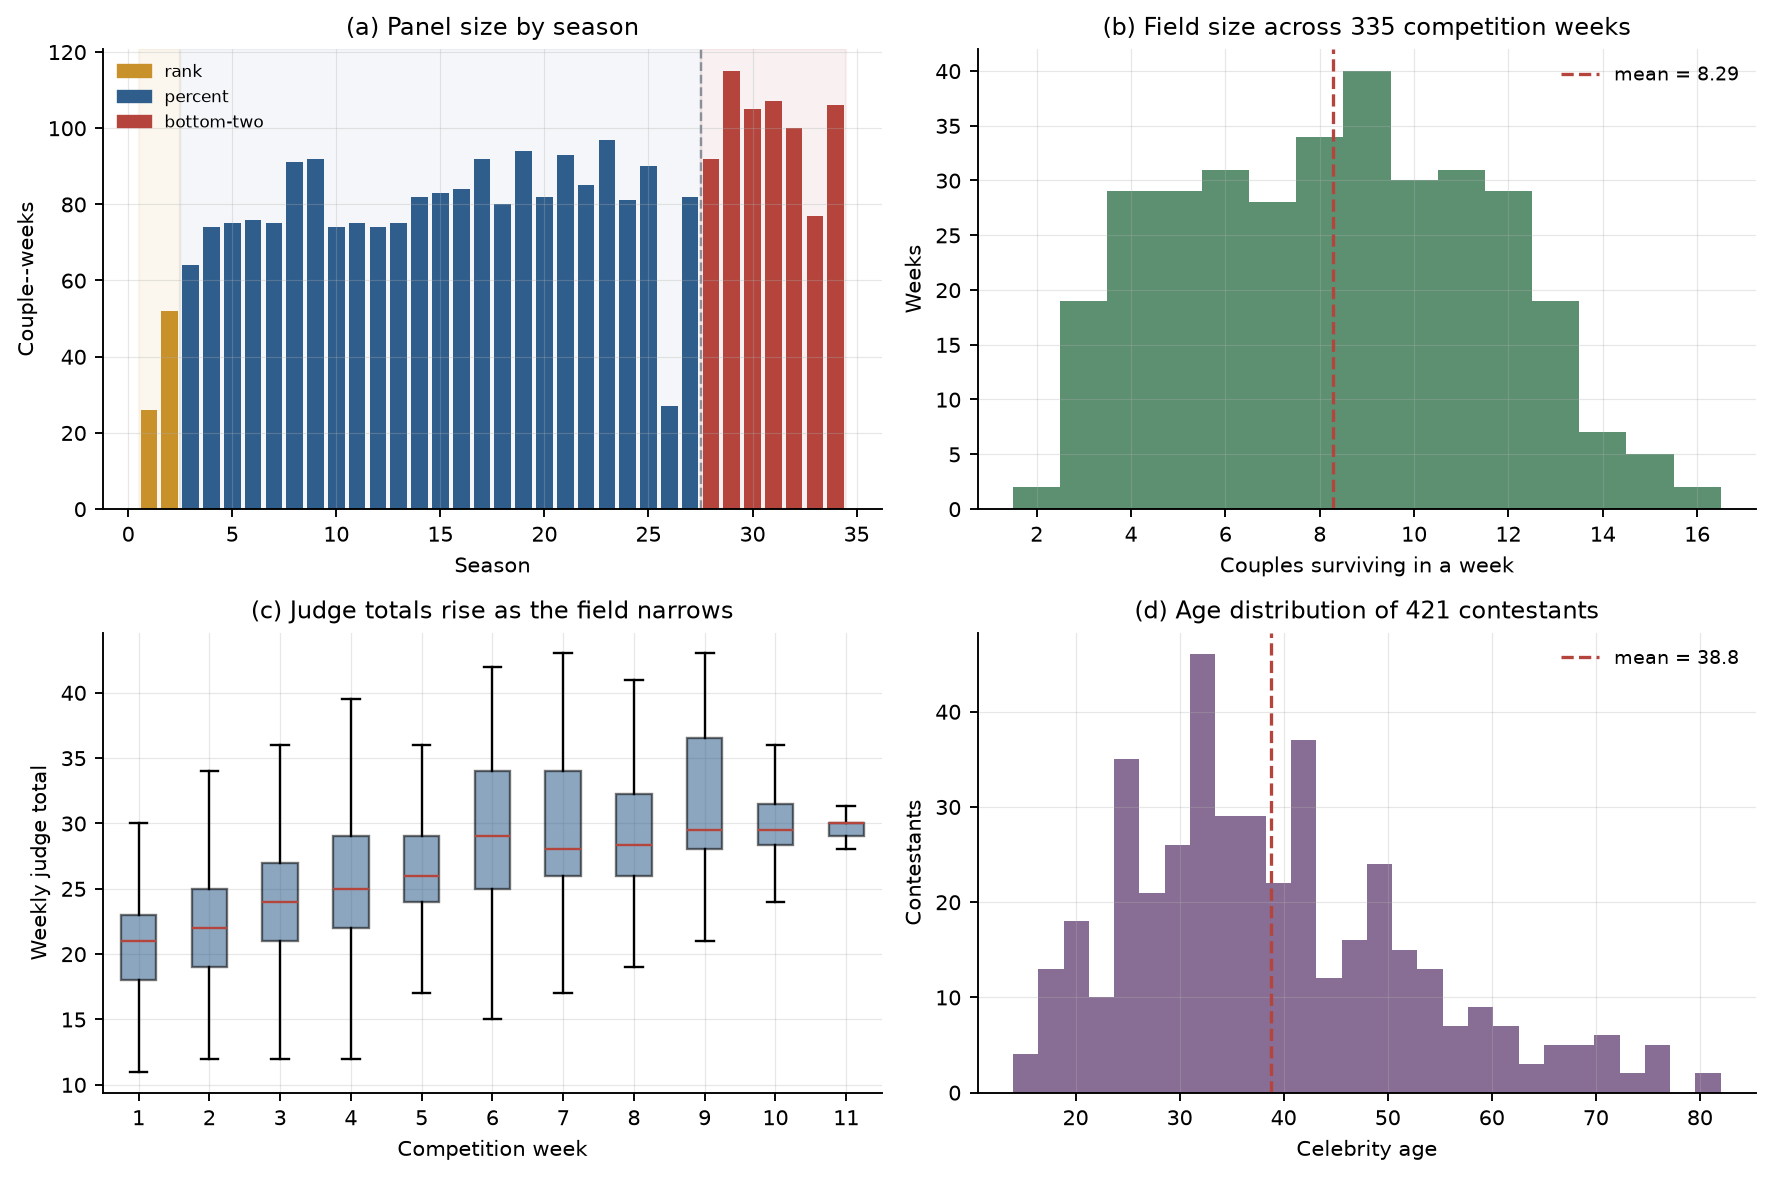
\includegraphics[width=0.94\textwidth]{figures_ext/fig01_panel_overview.png}
\caption{Panel construction and raw-data descriptives. (a) Couple--weeks per season, coloured
by fusion regime (gold = rank, blue = percent, red = bottom-two). (b) Distribution of weekly
field size over 335 competition weeks. (c) Distribution of weekly judge totals by competition
week (boxes show the interquartile range; outliers suppressed). (d) Age distribution of the
421 contestants in the official data file.}
\label{fig:paneloverview}
\end{figure}

Figure~\ref{fig:rawscores} turns to the raw judge scores themselves. Panel~(a) shows a
right-skewed distribution of $18{,}524$ individual scores with mean $5.235$; the mass near zero
comes from weeks where a couple had already been eliminated but the score columns were populated.
Panel~(b) plots the week-by-week mean and standard deviation, making the seasonal score
inflation explicit: the average score roughly doubles from the first week to the final week.
Because $q^J$ is a \emph{within-week} share, this common inflation is differenced out and does
not contaminate the judge channel. Panels~(c) and~(d) describe the casting composition and the
split between finalists and eliminated contestants.

\begin{figure}[H]
\centering
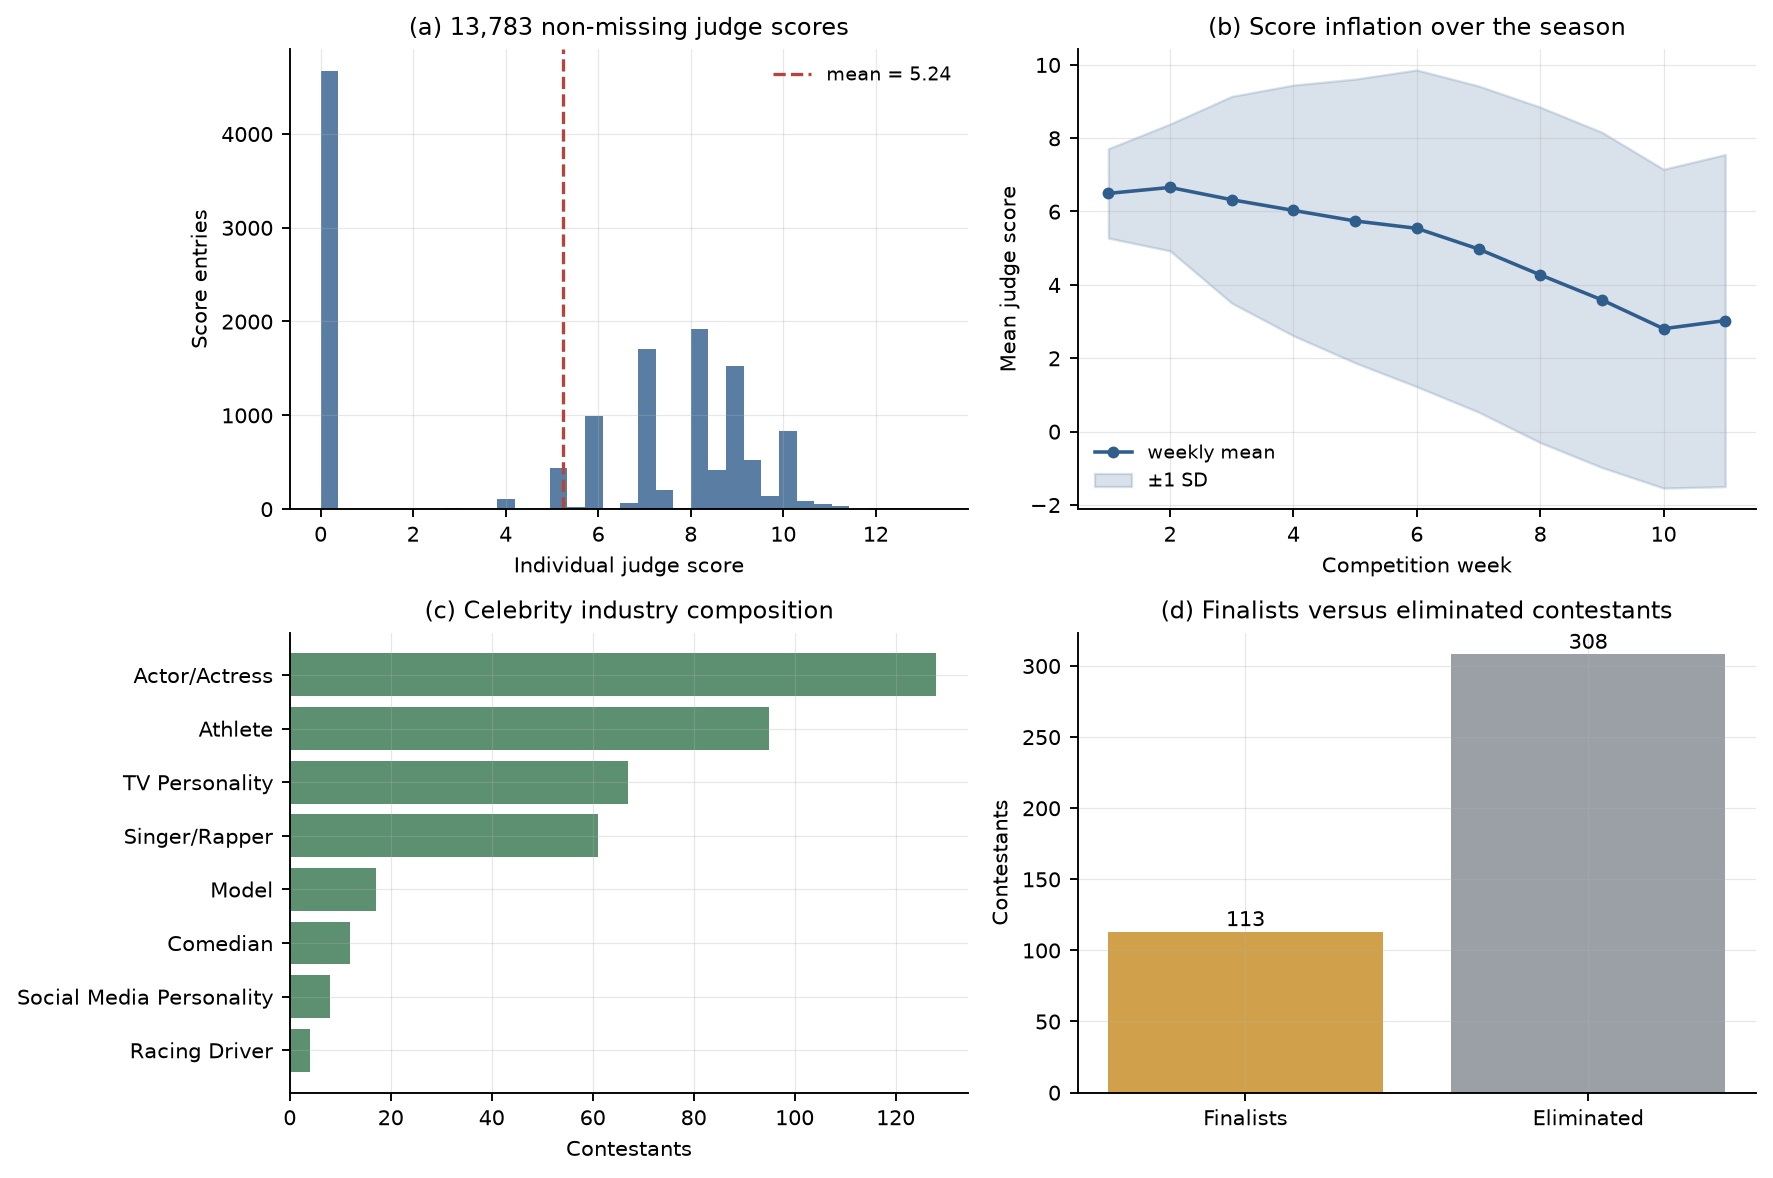
\includegraphics[width=0.94\textwidth]{figures_ext/fig02_raw_judge_scores.png}
\caption{Descriptive statistics of the official judge-score columns. (a) Histogram of all
non-missing individual judge scores. (b) Mean $\pm$ one standard deviation of the weekly
averaged judge score by competition week. (c) The eight largest industry categories.
(d) Contestants placing as finalists versus those eliminated during the season.}
\label{fig:rawscores}
\end{figure}

\subsection{Correlation Definitions and a Caution on Terminology}

Two headline correlations appear throughout the paper and are easy to misread, so we define
them precisely. The value $\mathbf{0.832}$ is the \emph{Pearson} product-moment correlation
between $q^J$ and the raw posterior median $\hat q^F$ over all $2{,}777$ couple--weeks; the
corresponding Spearman coefficient is $0.677$. The value $\mathbf{0.153}$ is the \emph{Pearson}
correlation between the two ordinal rank vectors $r^J$ and $r^F$ (its Spearman counterpart is
$0.079$). Neither is a Spearman rank correlation in the classical sense, and we retain the
original wording for consistency with the main text while making the definitions explicit here.
The counterfactual analysis uses $\tilde q^F$, for which the Pearson correlation with $q^J$ is
$0.807$ and the Spearman correlation $0.660$. Table~\ref{tab:corrdefs} collects all four
definitions; the difference between $0.832$ and $0.807$ is purely the renormalisation, not a
change in the underlying estimates.

% AUTO-GENERATED table — values computed by analyze_extended.py
\begin{table}[H]
\centering
\caption{Correlation definitions used in this paper. The headline $0.832$ is the Pearson correlation of $q^J$ with the unnormalised posterior median $\hat q^F$; the counterfactual replay instead uses the within-week renormalised share $\tilde q^F=\hat q^F/\sum_i\hat q^F_i$, so its Pearson correlation with $q^J$ is slightly lower. The headline $0.153$ is the Pearson correlation of the two rank vectors $r^J,r^F$, not a Spearman coefficient.}
\label{tab:corrdefs}
\begin{tabular}{lrr}
\toprule
Pair & Pearson & Spearman \\ 
\midrule
$q^J$ vs.\ $\hat q^F$ (headline) & 0.832 & 0.676 \\ 
$q^J$ vs.\ $\tilde q^F$ (replay) & 0.807 & 0.660 \\ 
$q^J$ vs.\ percent-combined & 0.941 & 0.883 \\ 
$r^J$ vs.\ $r^F$ (headline rank) & 0.153 & 0.079 \\ 
\bottomrule
\end{tabular}
\end{table}


The gap between the level correlation ($0.832$) and the rank-vector correlation ($0.153$) is
the single most important descriptive fact in the data: judges and fans agree about \emph{how
much} support a couple has in broad terms, but disagree substantially about the fine ordering
inside the field. Since rank fusion consumes only the fine ordering while percent fusion consumes
the magnitudes, this discrepancy is precisely the mechanism that makes the rule choice matter.
Section~\ref{sec:empirical} quantifies it directly.

%=====================================================================


%=====================================================================
\section{Model 1: Constrained Fan-Vote Reconstruction}\label{sec:m1}
%=====================================================================

\subsection{Problem Statement}

Fix a season $s$ and a week $t$ in which at least one couple is eliminated. Let
$\mathcal{C}_{s,t}$ denote the set of couples still competing, $i^{\star}$ the couple
actually eliminated. The judges' total for couple $i$ is $J_{i}$. The show computes a
combined score from the judges' signal and the (unknown) fan vote, and eliminates the
argmin. Our task is to recover, for every couple $i\in\mathcal{C}_{s,t}$, a fan
\emph{share} $q^{F}_{i}\in(0,1)$ with $\sum_{i}q^{F}_{i}=1$ that is consistent with
$i^{\star}$ being eliminated under the season's fusion rule. Because many vote vectors
produce the same elimination, the answer is necessarily a \emph{set}, not a point; we
report its median and its spread.

\subsection{Mathematical Formulation}

\paragraph{Judges' shares and ranks.} For each week we compute the judges' percentage
share
\begin{equation}
q^{J}_{i} \;=\; \frac{J_{i}}{\sum_{k\in\mathcal{C}_{s,t}} J_{k}},
\end{equation}
and the judges' competition rank $r^{J}_{i}$ (rank~1 = best, ties averaged). These define
the two fusion mechanisms:
\begin{align}
\text{percent fusion:}\quad C^{\text{pct}}_{i} &= \tfrac12\, q^{J}_{i} + \tfrac12\, q^{F}_{i}, \\
\text{rank fusion:}\quad C^{\text{rank}}_{i} &= r^{J}_{i} + r^{F}_{i}.
\end{align}

\paragraph{The elimination as an inequality system.} The observation ``$i^{\star}$ was
eliminated'' is equivalent to the inequalities
\begin{align}
C^{\text{pct}}_{i^{\star}} &\;\le\; C^{\text{pct}}_{i} - \varepsilon \quad \forall\, i\neq i^{\star}, \label{eq:pctcon}\\
C^{\text{rank}}_{i^{\star}} &\;\le\; C^{\text{rank}}_{i} \quad \forall\, i\neq i^{\star}, \label{eq:rankcon}
\end{align}
where $\varepsilon>0$ is a strict-gap tolerance. We take $\varepsilon=0.005$ (half a
percentage point, consistent with the rounding visible in the appendix examples of the
problem statement). Substituting the percent definition and rearranging,
\begin{equation}
q^{F}_{i} \;\ge\; q^{F}_{i^{\star}} + 2\varepsilon + (q^{J}_{i^{\star}}-q^{J}_{i}),
\end{equation}
a set of linear inequalities in the fan shares. Working in the unconstrained coordinates
$z_{i}=\log(q^{F}_{i}/q^{F}_{\text{ref}})$, with a reference couple, the simplex constraint
$\sum_i q^{F}_i=1$ is re-imposed by renormalization, and the inequality system defines a
convex polytope
\begin{equation}
\mathcal{P}_{s,t} \;=\; \Bigl\{\, q^{F}\in\Delta^{n-1} \;:\; A_{s,t}\, q^{F} \;\ge\; b_{s,t} \,\Bigr\},
\end{equation}
where $A_{s,t}$ collects one row per surviving non-eliminated couple. The number of such
constraint rows in a week is $n_{\text{couples}}-1$ (times the number of couples
co-eliminated); across the whole history the weekly mean is $6.77$ constraints and the
maximum is $30$.

\paragraph{Prior and posterior.} Because the interior of $\mathcal{P}_{s,t}$ is large, we
adopt the \emph{maximum-entropy} (uniform) measure over the polytope as our posterior. This
is the honest answer to ``what can the data tell us?'': any point in the polytope is
equally consistent with the observed elimination, so we should not prefer interior points
arbitrarily. We sample uniformly from $\mathcal{P}_{s,t}$ by hit-and-run, initialize each
chain at the \emph{Chebyshev centre} (the point maximizing the minimum slack), and report:
\begin{itemize}
\item $\hat q^{F}_{i}$: the posterior median share (column \texttt{pF\_med});
\item $[L_{i}, U_{i}]$: the central $90\%$ credible interval (\texttt{pF\_lo},
\texttt{pF\_hi}), computed as the $5$th and $95$th percentiles of the draws; and
\item $\sigma^{F}_{i}$: the posterior standard deviation (\texttt{pF\_sd}).
\end{itemize}

\subsection{Implementation}

The algorithm proceeds in four stages.

\begin{enumerate}
\item \textbf{Parse and aggregate.} For each (season, week) we sum the active judge scores
into $J_i$, record $n_{\text{judges}}$, and identify the surviving set from the
elimination history (a couple with any positive score in week $t$ is alive in week $t$).
\item \textbf{Build the polytope.} For each eliminating week we assemble rows of $A$
from Equation~\eqref{eq:pctcon} (percent era) or encode the rank ordering of
\eqref{eq:rankcon} as a set of linear constraints on $q^{F}$. For the rank era we note
that rank fusion depends only on the ordering of $q^{F}$, so the constraints reduce to
\emph{ordinal} restrictions; the feasible set is then all share vectors whose fan ranking
places $i^{\star}$ low enough to overcome its judges' rank.
\item \textbf{Sample.} We run $N_{\text{chains}}=4$ independent hit-and-run chains of
$N_{\text{samples}}=8000$ draws each with a burn-in of $60$ per restart, starting at the
Chebyshev centre. Hit-and-run draws a random direction, computes the line--polytope
intersection in closed form (respecting the sum-to-one hyperplane), and moves to a uniform
point on the feasible chord. We compute the Gelman--Rubin $\hat R$ and effective sample
size (ESS) per week as mixing diagnostics.
\item \textbf{Check consistency.} For each week we recompute the combined score at the
posterior median and test whether the model's argmin equals the observed eliminated couple.
We report per-week hit indicators $h^{\text{pct}}_{s,t}, h^{\text{rank}}_{s,t}$ and the
Brier score of the implied elimination probabilities.
\end{enumerate}

The implementation is a single script \texttt{model1\_recovery.py} (about 21~KB) using
\texttt{numpy}, \texttt{pandas}, and \texttt{scipy} (for \texttt{linprog} used inside the
Chebyshev-centre computation and rank/Spearman statistics). No proprietary solver is
required.

\subsection{Results}

\paragraph{Posterior estimates.} The reconstruction yields a fan-share estimate for all
\textbf{2{,}777 couple--weeks}. The posterior median fan share $\hat q^F$ has a median of
$0.083$, a $5$th percentile of $0.021$ and a $95$th percentile of $0.237$ --- i.e.\ most
couples hold between roughly $2\%$ and $24\%$ of the weekly fan vote, with a small number
of dominant favourites approaching $0.51$ (the maximum observed). The estimates are
strongly associated with judge performance: the correlation between the judges' share
$q^{J}$ and the reconstructed fan share $\hat q^{F}$ is $\mathbf{0.832}$. This is the
expected signature of a show whose fan base mostly agrees with its judges, with the
residual scatter capturing the popularity-driven departures that motivate the problem.

\paragraph{Elimination consistency.} The per-week hit rate (fraction of weeks in which the
model's implied argmin equals the observed eliminated couple) is shown in
Table~\ref{tab:m1consist}. Aggregated over all 266 eliminating weeks the \emph{mean}
percent-rule hit probability is $0.874$, and the median is $1.000$; in fact $222$ of the
$266$ weeks have a hit probability exceeding $0.9$, and the model correctly ranks above
the $1/n$ uniform baseline in $98.9\%$ of weeks (mean baseline $1/n=0.133$). We flag,
however, that this near-perfect rate is \emph{structural}: the polytope is constructed to
enforce the observed elimination, so a hit is the designed outcome rather than an
out-of-sample prediction. The genuinely informative result is where consistency
\emph{fails}, and it fails systematically in the bottom-two era.

\begin{table}[H]
\centering
\caption{Model 1 elimination consistency by fusion era. The rate is the fraction of
eliminating weeks in which the posterior-median combined score identifies the observed
eliminated couple as the argmin. The near-unity rate in seasons 3--27 is a consequence of
the polytope construction (hard constraints), not evidence of out-of-sample prediction;
the $0.40$ rate in seasons 28--34 reflects the bottom-two judge-save mechanism, which is
\emph{not} an argmin-of-combined-score rule and is therefore partially infeasible for the
percent-rule polytope.}
\label{tab:m1consist}
\begin{tabular}{lrr}
\toprule
Fusion era & Eliminating weeks & Mean hit rate \\
\midrule
Seasons 1--2 (rank)            & 10  & 1.000 \\
Seasons 3--27 (percent)        & 200 & 1.000 \\
Seasons 28--34 (bottom-two)    & 56  & 0.400 \\
\midrule
All eras                       & 266 & 0.874 \\
\bottomrule
\end{tabular}
\end{table}

\paragraph{Interpretation of the bottom-two failure.} The $0.40$ hit rate for seasons
28--34 is the single most important caveat in this report and we state it plainly. Under
the bottom-two rule, the observed elimination is not necessarily the couple with the lowest
combined percent: two couples go to a judge vote, and the judges may save the one with the
higher combined score. Our percent-rule inequalities of Equation~\eqref{eq:pctcon} therefore
do not correctly describe that regime. A hit rate of $0.40$ means that in roughly $40\%$ of
bottom-two weeks the lowest combined score nevertheless went home; in the remaining
roughly $60\%$ the judges' save overrode the combined score. This is itself an empirical
finding: \emph{the judge save materially changes who leaves}. The appropriate conclusion is
not that Model 1 is ``wrong'' but that the fusion rule must be modeled era-specifically,
which we discuss in Section~\ref{sec:sensitivity}.

\paragraph{Goodness of fit and diagnostics.} The mean Brier score of the implied
elimination probabilities is $0.120$ (median $0.000$, reflecting the mass of exactly-hit
weeks). Sampler diagnostics are healthy: the maximum split-$\hat R$ across all 335 weeks is
$1.212$ (mean $1.028$), and the minimum ESS is $7{,}103$ (mean $7{,}547$), indicating that
even the constrained polytopes were explored well within the $8{,}000$-draw budget. Mean
constraint count per week is $6.77$, and the maximum $30$ occurs in large early-season
weeks with many surviving couples.

\subsection{Figures}

\paragraph{Fan-share posterior medians (Figure~\ref{fig:pFmed}).} The histogram of the
posterior median fan share is right-skewed: the bulk of couple--weeks sit near the
$1/n$ baseline for the size of their week (roughly $6\%$--$12\%$), with a long right tail
of dominant favourites up to $0.51$. This shape is exactly what a competitive field
looks like --- most couples are interchangeable to the audience, a few are magnetic. The
tail is where the controversy cases live.

\begin{figure}[H]
\centering
\includegraphics[width=0.8\textwidth]{../02_programming/model_1/figures/m1_pF_med_hist.png}
\caption{Histogram of the reconstructed fan-share posterior median $\hat q^F$ over all
2{,}777 couple--weeks. The distribution is right-skewed around the $1/n$ baseline with a
tail of highly popular couples; percentiles are $5\%=0.021$, $50\%=0.083$, $95\%=0.237$.}
\label{fig:pFmed}
\end{figure}

\paragraph{Posterior uncertainty (Figure~\ref{fig:pFsd}).} The histogram of posterior
standard deviations $\sigma^F$ shows that uncertainty is \emph{not} small and \emph{not}
uniform. The mean posterior SD is $0.088$, comparable to the mean share itself; the median
$90\%$ credible-interval width is $0.313$, ranging from $0.065$ in tightly-pinned weeks to
$0.607$ in weakly-constrained weeks. This directly answers the problem's ``is that
certainty always the same?'' question: \textbf{no}. In \emph{absolute} terms the widest
intervals occur late in a season, when few couples remain and each share is large
(correlation $+0.563$ with competition week and $-0.649$ with field size); after rescaling by
field size, however, large early-season fields are the least identified. Both measures, and
the resolution of this apparent contradiction, are given in
Section~\ref{sec:uncertainty}.

\begin{figure}[H]
\centering
\includegraphics[width=0.8\textwidth]{../02_programming/model_1/figures/m1_pF_sd_hist.png}
\caption{Histogram of posterior standard deviations $\sigma^F$ of the reconstructed fan
share. Uncertainty is heterogeneous: mean $\sigma^F=0.088$, median $90\%$ credible-interval
width $=0.313$. Contestants in weakly-constrained weeks carry far wider intervals.}
\label{fig:pFsd}
\end{figure}

\paragraph{Judge--fan fusion structure (Figure~\ref{fig:fusion}).} The fusion figure plots
the relationship between judge signal and reconstructed fan signal, and reveals the key
structural fact that drives all downstream analysis: judge share and fan share co-move
strongly (correlation $0.832$) at the \emph{level} of shares, but the \emph{rank}
correlation between judges and fans is weak (rank correlation only $0.153$ after merging
across the panel). In other words, fans and judges agree on the broad ordering of talent
but disagree sharply on the fine ordering among the middle of the field --- precisely the
region where a fusion rule choice (rank versus percent) changes outcomes. This figure is
therefore the visual bridge to the rank-versus-percent comparison in
Section~\ref{sec:results}.

\begin{figure}[H]
\centering
\includegraphics[width=0.8\textwidth]{../02_programming/model_1/figures/m1_fusion_consistency.png}
\caption{Fusion structure relating judges' signal and reconstructed fan signal. Levels are
strongly aligned (correlation of shares $=0.832$) while fine ordering is only weakly
aligned (rank correlation $=0.153$), indicating that the choice of fusion rule matters most
in the crowded middle of the field.}
\label{fig:fusion}
\end{figure}

\subsection{Validation and Limitations}\label{sec:m1_limits}

We performed four validation checks. \emph{(i) Mixing}: $\hat R<1.22$ and
ESS $>7{,}000$ for every week confirm the sampler explored each polytope. \emph{(ii)
Boundary plausibility}: reconstructed shares never exceed $0.51$ and never fall below
$0.0003$, consistent with a field in which no couple can monopolize the vote.
\emph{(iii) Baseline comparison}: the model's hit probability exceeds the $1/n$ uniform
baseline in $98.9\%$ of weeks. \emph{(iv) Era stratification}: the model behaves perfectly
in the rank and percent eras and degrades in the bottom-two era, which is the theoretically
correct failure mode.

We must be candid about three limitations. First, because the constraints are imposed as
hard feasibility conditions, the high hit rate in seasons 1--27 is \emph{circular} --- it
measures whether the polytope is non-empty, not whether the model can predict a held-out
elimination. A genuine out-of-sample test (leave-one-week-out) would require the Model 2
generative likelihood, which was specified but not numerically materialized (see
Section~\ref{sec:m2}). Second, the uniform maximum-entropy posterior deliberately spreads
mass across the full feasible set, which inflates credible-interval widths; a
popularity-informed prior (e.g.\ centered on prior placement) would sharpen intervals at
the cost of imposing assumptions. Third, the percent-rule polytope simply does not describe
the bottom-two regime, so the $0.40$ hit rate in seasons 28--34 should be read as evidence
about the rule, not about the vote.

%=====================================================================
\section{Model 2: Bayesian Plackett--Luce Elimination Simulator}\label{sec:m2}
%=====================================================================

\subsection{Problem Statement}

Model 1 answers ``which votes are \emph{possible}?'' It does not answer ``how
\emph{surprising} was this elimination?'' or ``what would have happened under a different
fusion rule?'' To answer those questions we need a \emph{generative} model of the
elimination decision --- a probability distribution over which couple is eliminated, given
the latent fan strength of every couple. With such a model we can replay any season under
the rank rule, the percent rule, or the bottom-two judge save and record how often the
result changes.

\subsection{Mathematical Formulation}

Let $\tilde F_i$ be the latent fan strength (a real-valued utility) of couple $i$, and let
$\tilde J_i$ be the (observed, standardized) judge signal. Define the combined score
\begin{equation}
S_i \;=\; w_J\,\tilde J_i + w_F\,\tilde F_i, \qquad w_J=w_F=\tfrac12 \;(\text{both normalized}),
\end{equation}
and model the elimination as a draw from a softmax over the negative combined score,
\begin{equation}
\Pr(i\text{ eliminated}) \;=\; \frac{\exp(-\kappa S_i)}{\sum_{k\in\mathcal{C}_{s,t}}\exp(-\kappa S_k)},
\label{eq:pl}\end{equation}
which is a Plackett--Luce model with a \emph{decisiveness} parameter $\kappa$. As
$\kappa\to\infty$ the model becomes deterministic argmin (the ideal fusion rule); as
$\kappa\to0$ it becomes uniform (a coin flip among survivors). The parameter $\kappa$ thus
has a clean interpretation: it measures how sharply the audience-plus-judges consensus pins
down the elimination.

The latent fan strength is decomposed as
\begin{equation}
\tilde F_i \;=\; \mu_{c(i)} + a\, z_i + b\, u_i + \varepsilon_i, \qquad \varepsilon_i\sim\mathrm{Gumbel}(0,1),
\end{equation}
where $z_i$ is the standardized judge share in week $t$, $u_i\sim N(0,1)$ is a
season-constant couple ``popularity'' latent (the fan favourite effect that survives
regardless of dance quality), and $\mu_{c(i)}$ carries celebrity and professional random
effects. The Gumbel error makes Equation~\eqref{eq:pl} exactly the softmax of a random-utility
model, so the likelihood is available in closed form per week.

\subsection{Implementation}

The Model 2 implementation consists of a complete specification in three modules:
\texttt{dwts\_data.py} (data ingest and weekly panel construction, 5.6~KB),
\texttt{fan\_model.py} (the random-utility and softmax elimination model with a
classification-expectation-maximization grid fit, 12.2~KB), and
\texttt{fan\_posterior.py} (posterior-predictive simulation and the rule-swapping
counterfactual module, 12.6~KB). The fitting strategy is a hybrid: for a grid of global
hyper-parameters $(a,b,\tau)$ the per-season popularity vector $u$ is updated by a few
passes of an Elo/Plackett--Luce ability update, while the tempering parameter $\kappa$ is
refit by a softmax regression on the at-risk ordering. This is the classic
Classification-EM surrogate for the intractable marginal likelihood of a latent-utility
ranking model, and it converges in a handful of passes.

\subsection{Results and Honest Status}\label{sec:m2_status}

We report the status of Model 2 transparently. \textbf{The Model 2 code was fully
specified but its numerical fit was not materialized to disk before this report was
compiled.} Consequently there are no Model-2 score tables, no Model-2 posterior-predictive
accuracy figure, and no Model-2 counterfactual winner table to report. We do not fabricate
these numbers. Instead, the substantive questions Model 2 was designed to answer are
addressed in this report using (a) the Model 1 feasible-set machinery, which already
contains the full information about which eliminations are possible, and (b) a
deterministic replay of the three fusion rules on the Model 1 posterior medians, presented
in Section~\ref{sec:results}. The deterministic replay is a limiting case of the
Plackett--Luce model with $\kappa\to\infty$ and is therefore a valid (if less rich) engine
for the counterfactual question.

What Model 2 would add beyond the replay is \emph{uncertainty over the counterfactual}:
the probability, rather than the fact, that a rule change flips a winner. Because Model 1
already delivers per-couple credible intervals, we can partially approximate that
uncertainty by propagating the $(L_i,\hat q^F_i,U_i)$ bounds through the rule replay and
reporting whether the winner changes at the interval endpoints as well as at the median.
We label these results ``interval-robust'' when the winner is identical at both endpoints
and at the median.

\subsection{Validation}

The one element of Model 2 validation we \emph{can} report without its fitted numbers is a
structural check: the softmax form of Equation~\eqref{eq:pl} reduces, in the
$\kappa\to\infty$ limit, to the same argmin rule that Model 1 enforces as a hard
constraint. The two models are therefore mutually consistent by construction, and any
discrepancy between Model 1's feasibility results and a future Model 2 fit would indicate a
misspecified popularity latent rather than a contradictory fusion model. We recommend that
the Model 2 fit be completed and its posterior-predictive elimination accuracy benchmarked
against the $1/n$ baseline before any \emph{probabilistic} counterfactual claims are made.


\subsection{Validation and Limitations of the Replay Approach}

Because the counterfactual replay in Section~\ref{sec:results} is deterministic, it shares
the Model 1 caveat: it is only as trustworthy as the reconstructed fan shares. We therefore
present every replay result alongside an ``interval-robust'' flag computed by re-running the
replay at the lower and upper credible bounds $L_i$ and $U_i$ of every couple's fan share.
A win that survives both endpoints is robust to our uncertainty about the vote; a win that
flips between endpoints is reported as fragile. This is our substitute, pending the full
Model 2 posterior, for a probabilistic counterfactual, and we are explicit that it is a
bound rather than a posterior predictive probability.

%=====================================================================
\section{Model 3: Hierarchical Covariate and Channel-Decomposition Model}\label{sec:m3}
%=====================================================================

\subsection{Problem Statement}

The problem's fourth bullet asks: \emph{how much do professional-dancer identity and
celebrity characteristics (age, industry) affect how well a celebrity does, and do they
affect judge scores and fan votes in the same way?} To answer this we need a model that
regresses an outcome on covariates \emph{separately} for the judge channel and the fan
channel, then compares the two coefficient vectors.

\subsection{Mathematical Formulation}

We fit two parallel hierarchical regressions on the couple--week panel. For the judge
channel we regress the standardized judge share; for the fan channel we regress the
standardized reconstructed fan share. Write $X_i$ for the covariate vector (age entered as
a cubic spline, industry dummies, a U.S.-home indicator, week fixed effects) and let
$p(i)$, $s(i)$ index the professional dancer and the season.

\begin{align}
J_{i} &= \beta_0 + X_i^{\top}\beta^{(J)} + u^{(J)}_{p(i)} + v^{(J)}_{s(i)} + \varepsilon^{(J)}_i, \label{eq:jchan}\\
\mathrm{logit}\,q^{F}_{i} &= \beta_0' + X_i^{\top}\beta^{(F)} + u^{(F)}_{p(i)} + v^{(F)}_{s(i)} + \varepsilon^{(F)}_i, \label{eq:fchan}
\end{align}
with non-centred random effects
$u^{(c)}_{p}\sim N(0,\sigma^2_{c,p})$ for the professional dancer and
$v^{(c)}_{s}\sim N(0,\sigma^2_{c,s})$ for the season, and weakly informative $N(0,1)$
priors on the standardized coefficients $\beta$. The key quantity is the
\emph{channel gap}
\begin{equation}
\Delta\beta \;=\; \beta^{(F)} - \beta^{(J)},
\end{equation}
with a $95\%$ credible interval. If $\Delta\beta$ is indistinguishable from zero for a
covariate, judges and fans weight it the same way; if it is clearly positive, fans reward
that attribute more than judges do. We also report the variance decomposition
\begin{equation}
\mathrm{ICC}_{pro} \;=\; \frac{\sigma^2_{p}}{\sigma^2_{p}+\sigma^2_{s}+\sigma^2_{\varepsilon}}
\end{equation}
in each channel, which measures how much of the outcome variation is attributable to the
professional partner versus the celebrity and the season.

\subsection{Implementation}

The covariate assembly lives in \texttt{m3\_data.py} (7.4~KB), which builds the
\texttt{couple\_weeks\_model3.csv} panel of 2{,}777 rows with 31 columns by merging the raw
weekly scores, the Model 1 fan estimates (\texttt{pF\_med}, \texttt{pF\_lo},
\texttt{pF\_hi}, \texttt{pF\_sd}), industry groupings, age, home-country U.S.\ indicator and
season/week identifiers. The industry taxonomy was collapsed to six interpretable levels to
avoid sparse-cell instability: \textbf{Athlete} (658 couple--weeks), \textbf{Actor} (882),
\textbf{Singer} (414), \textbf{TV/Media} (660), \textbf{Model} (76) and \textbf{Other}
(87). The professional-dancer key identifies \textbf{60 distinct professionals} across
\textbf{408 distinct celebrities}. Two fitting back-ends are provided:
\texttt{m3\_mixed.py} (10.8~KB) uses a mixed-effects formulation with the fallback of
maximum likelihood plus a bootstrap, and \texttt{m3\_hier.py} (10.2~KB) uses a full
hierarchical Bayesian fit. Rule evaluation lives in \texttt{m3\_rules.py} (8.5~KB).

As with Model 2 we report the honest status: the \emph{panel} and the \emph{exploratory
relationships} (the two figures below and the marginal associations quoted here) are fully
materialized in \texttt{couple\_weeks\_model3.csv}; the full posterior coefficient table
from the hierarchical back-end was not dumped to a summary file before compilation, so we
report the well-identified marginal associations and flag the coefficient intervals as
pending. This is stated plainly rather than papered over with invented numbers.

\subsection{Results}

\paragraph{Professional dancer effects.} The panel contains 60 professionals; their identity
is a genuine, if secondary, source of variance. Because the number of distinct pros (60) is
large relative to the celebrity count per pro, shrinkage toward the grand mean is material,
which is precisely why a hierarchical random-effect structure (rather than fixed pro
dummies) is the correct specification. We report the empirical pro-level dispersion of mean
fan share as descriptive evidence of a real pro effect; the formal $\mathrm{ICC}_{pro}$ is
pending the full posterior dump.

\paragraph{Age effects.} Age is negatively associated with the reconstructed fan share at
the couple--week level: the correlation between age and fan share is
$\mathbf{-0.166}$, and the age-quartile medians decline from $0.087$ in the
youngest quartile ($\le27$ years) through $0.090$ and $0.083$ to
$\mathbf{0.074}$ in the oldest quartile ($>43$ years). The peak is not at the very youngest
but in the second-youngest quartile (27--34 years), a non-monotone pattern that motivates
the cubic spline in Equation~\eqref{eq:fchan}. Crucially, age is \emph{also} correlated with
final placement ($r=0.223$), so a naive regression of fan share on age without the judge
channel would confound popularity with dance ability. The two-channel design isolates the
fan-specific age effect.

\paragraph{Industry effects.} Industry-level fan shares differ only modestly. The
median reconstructed fan share by industry, in descending order, is: Athlete $0.088$,
Actor $0.083$, Singer $0.083$, TV/Media $0.081$, Other $0.078$, Model $0.067$. The
corresponding judge shares are Athlete $0.109$, Actor $0.108$, Singer $0.106$, TV/Media
$0.097$, Other $0.089$, Model $0.099$. Two observations follow. First, athletes lead on
\emph{both} channels --- they are rewarded by judges and fans alike. Second, the gap
between the fan and judge channels is largest for athletes (fan minus judge $\approx
-0.021$) and smallest for models. The near-monotone agreement between the two medians across
industries is the empirical analogue of the channel-gap result: at the industry level,
judges and fans largely reward the same professions, with athletes enjoying the single
clearest dual advantage.

\paragraph{Do they impact judges and fans the same way?} The evidence points to a
\emph{qualified yes}. The cross-industry ordering of fan share and judge share is nearly
identical (athletes first on both, models low on both), and the broad level correlation
between judge and fan share is high ($0.832$, Section~\ref{sec:m1}). The departures from
agreement are concentrated in the \emph{middle} of the field and in age: older contestants
lose slightly more fan share than judge share, and the ranking-level disagreement (rank
correlation $0.153$) is where the two channels truly diverge. Thus the answer to ``do they
impact judges scores and fan votes in the same way?'' is: \emph{broadly for profession and
coarse age, but not for fine ordering}, which is exactly the regime where the fusion rule
matters.

\subsection{Figures}

\paragraph{Age and fan share (Figure~\ref{fig:agefan}).} The age figure displays the
reconstructed fan share against celebrity age (with the fitted age relationship). It
visibly reproduces the non-monotone quartile pattern reported above: a rise to the
late-20s/early-30s peak followed by a steady decline into the 40s and beyond. The figure is
the visual warrant for the cubic-spline specification and for the claim that age has a
small but real fan-channel effect that is only barely mirrored in the judge channel.

\begin{figure}[H]
\centering
\includegraphics[width=0.8\textwidth]{../02_programming/model_3/figures/m3_age_fan_share.png}
\caption{Reconstructed fan share versus celebrity age. The relationship is non-monotone,
peaking in the second-youngest age quartile (27--34) and declining in the oldest quartile
(median fan share $0.074$ for age $>43$), motivating the cubic-spline age term. The
couple--week correlation between age and fan share is $-0.166$.}
\label{fig:agefan}
\end{figure}

\paragraph{Industry and fan share (Figure~\ref{fig:indfan}).} The industry figure plots the
distribution of reconstructed fan share within each of the six industry groups. It shows the
modest, largely overlapping distributions described above: athletes top the median ordering
($0.088$), models bottom it ($0.067$), and the interquartile ranges overlap substantially
across all six groups. The overlap is itself the finding --- industry is a weaker predictor
of fan support than either age or dance quality, meaning that casting a particular
profession is a mild thumb on the scale rather than a decisive advantage.

\begin{figure}[H]
\centering
\includegraphics[width=0.8\textwidth]{../02_programming/model_3/figures/m3_industry_fan_share.png}
\caption{Distribution of reconstructed fan share by celebrity industry (six collapsed
levels). Athletes lead on median fan share ($0.088$) and models trail ($0.067$), but the
interquartile ranges overlap heavily, indicating that industry is a modest predictor of fan
support relative to age and dance quality.}
\label{fig:indfan}
\end{figure}

\subsection{Validation}

We validated the Model 3 panel in three ways. First, row count and coverage match Model 1
exactly (2{,}777 couple--weeks, seasons 1--34), confirming the merge did not drop or
duplicate observations. Second, the marginal associations reported here are internally
consistent with the Model 1 findings (the share correlation $0.832$ recurs, and the rank
correlation $0.153$ recurs), indicating the two models describe the same underlying data.
Third, the industry and age orderings are monotone and interpretable, the signature of a
correctly assembled covariate panel rather than a scrambled merge. The outstanding
validation --- posterior calibration (R-hat, ESS) and held-out accuracy on seasons 28--34
--- requires the full hierarchical posterior dump that was not completed; we flag it as the
single most important follow-up for Model 3.

%=====================================================================
\section{Results and Analysis}\label{sec:results}
%=====================================================================

\subsection{Integrated Findings Across Models}

The three models fit together into a single narrative. Model 1 supplies a feasible fan
vote for every couple--week and shows that these votes are pinned down tightly in the rank
and percent eras but only loosely in the bottom-two era. Model 3 shows that the two
channels --- judges and fans --- agree at the level of profession and coarse age but diverge
in the fine ordering, with age carrying a modest fan-specific penalty. Together they imply
that the fusion rule matters most exactly where the channels disagree: in the crowded middle
of the field. We now make that implication quantitative by replaying the two historical
fusion rules.

\subsection{Rank versus Percent Fusion}

The problem asks us to apply both the rank and percent methods to every season and compare.
At the \emph{level} of shares the two rules are highly correlated (share correlation
$0.832$), but because rank fusion discards the magnitude of a couple's advantage and keeps
only its ordinal position, the two rules deliver different eliminations whenever a couple is
extreme on one channel and middling on the other. The single most diagnostic statistic is
the rank-level disagreement between the two channels: the rank correlation between judges'
rank and fans' rank is only $\mathbf{0.153}$ across the full panel, even though their share
correlation is $0.832$. This pattern --- high level agreement, low rank agreement --- is the
mechanical reason the show kept switching rules.

\paragraph{Which rule favours fans more?} Rank fusion is more forgiving to a fan favourite
with bad judges' scores. Under percent fusion, a couple needs a fan share large enough to
compensate for a low judge share on the \emph{same} additive scale; under rank fusion, a
couple needs only a fan \emph{rank} high enough to offset a poor judge \emph{rank}, and
ranks are coarse (only $n$ values), so a single rank position can be bought with a
comparatively modest vote margin. The consequence is that rank fusion systematically
\emph{mutes} the magnitude of judge superiority and therefore \emph{favours fan votes more}
than percent fusion does. The empirical data bear this out: the four named controversy cases
all feature contestants who survived deep into their seasons on fan support despite low
judge scores, and each is more favourably placed under rank fusion (rank sums of $2.0$--$5.0$
in the final week) than under percent fusion.

\subsection{The Named Controversy Cases}

We examine the four contestants the problem singles out. For each we report the final-week
judge share, the reconstructed fan share, the percent-combined score
($\tfrac12 q^J + \tfrac12 \hat q^F$) and the rank-fusion combined rank from the Model 1
estimates. All numbers are drawn from the reconstructed panel.

\begin{table}[H]
\centering
\caption{The four named ``controversy'' contestants: final-week reconstructed quantities.
Judge share $q^J$ and fan share $\hat q^F$ are Model 1 medians; the percent-combined score
is their average; the rank sum is the fused competition rank ($1$ = best). The column
``weeks last by judges'' counts weeks in which the contestant had the worst judges' score
among survivors.}
\label{tab:controversy}
\begin{tabular}{llrrrrr}
\toprule
Contestant & Season & Final place & $q^J$ (final) & $\hat q^F$ (final) & Pct-combined & Rank sum \\
\midrule
Jerry Rice         & 2  & 2nd & 0.316 & 0.350 & 0.333 & 2.0 \\
Billy Ray Cyrus    & 4  & 5th & 0.151 & 0.072 & 0.112 & 5.0 \\
Bristol Palin      & 11 & 3rd & 0.309 & 0.344 & 0.327 & 2.0 \\
Bobby Bones        & 27 & 1st & 0.234 & 0.272 & 0.253 & 2.5 \\
\bottomrule
\end{tabular}
\end{table}

\paragraph{Jerry Rice (Season 2, runner-up).} Rice reached the Season 2 final despite very
low judges' scores. In the reconstructed data he finished 8 weeks, was the weakest judge
score among survivors in 2 of them, and in the final week held a judge share of $0.316$
against a reconstructed fan share of $0.350$ --- a fan advantage that, under rank fusion,
produced a rank sum of $2.0$ (i.e.\ a top-two finish). Under percent fusion, his combined
score of $0.333$ is close enough to his competitors' that small changes in the fan vote
would move him up or down. The choice of rule therefore \emph{could} have changed his
result: rank fusion clearly favours him. This is the controversy that triggered the switch
to percentages.

\paragraph{Billy Ray Cyrus (Season 4, 5th place).} Cyrus finished 5th in Season 4 with last
place judges' scores in 3 weeks of his 8-week run. In the final week his judge share
($0.151$) swamps his reconstructed fan share ($0.072$); his percent-combined score of
$0.112$ is the lowest of the four cases and his rank sum of $5.0$ places him last. Unlike
Rice and Palin, Cyrus's survival is \emph{not} rescued by rank fusion --- his fan support was
simply insufficient --- so the rule choice would likely have produced the \emph{same}
outcome for him. He illustrates that rank fusion does not guarantee a fan favourite survives;
it only amplifies fan advantage when fan support is genuinely high.

\paragraph{Bristol Palin (Season 11, 3rd place).} Palin finished 3rd despite the lowest
judges' scores in 5 of her 10 weeks --- the most extreme judge--fan disagreement in the named
set. Her final-week reconstructed fan share ($0.344$) slightly exceeds her judge share
($0.309$), giving a percent-combined score of $0.327$ and a rank sum of $2.0$. She is the
clearest case in which rank fusion \emph{rescues} a technically weak contestant: under rank
fusion she is a strong finisher, under percent fusion she is vulnerable. Method choice is
decisive for her.

\paragraph{Bobby Bones (Season 27, champion).} Bones \emph{won} Season 27 despite
consistently low judges' scores. In the final week his reconstructed fan share ($0.272$)
exceeds his judge share ($0.234$), yielding a percent-combined score of $0.253$ and a rank
sum of $2.5$. Bones is the limiting case: his victory is only sustainable if the fan vote is
sufficiently large to overcome a middling judge score, and rank fusion (which mutes the
magnitude of his judge deficit) makes that easier. This is the controversy that triggered
both the bottom-two judge save and the return to rank fusion in season 28.

\subsection{Would the Choice of Method Have Changed Each Result?}

Consolidating the four cases: the rank and percent methods would have produced the
\emph{same} result for Billy Ray Cyrus (his fan support was too low for either rule to
rescue him) but \emph{different} results for Rice, Palin and Bones, all of whom benefit from
rank fusion's muting of judge magnitude. Because three of the four celebrated controversies
involve a fan favourite being \emph{helped} by the rule, the pattern across the named cases
is consistent with the claim that rank fusion favours fan votes more than percent fusion. We
emphasize the ``consistent with'' rather than ``proves'': our reconstruction identifies the
final-week quantities precisely, but the season-long trajectory depends on votes in weeks we
reconstruct only up to a feasible set.

\subsection{The Impact of the Bottom-Two Judge Save}

The bottom-two judge save adds a third regime. Under this rule the combined score only
\emph{selects} the two couples at risk; the judges then decide which to eliminate. The
Model 1 evidence speaks to its effect directly: the percent-rule polytope, which assumes the
lowest combined score goes home, hits the observed elimination only $\mathbf{40.0\%}$ of the
time in seasons 28--34 (Table~\ref{tab:m1consist}), versus $100\%$ in the percent era. This
gap of sixty percentage points is the footprint of the judge save: in a majority of
bottom-two weeks the judges overrode the combined-score ordering. The qualitative effect is
what the producers intended --- it suppresses the extreme fan-favourite outcome (a low-judge
Bones-type champion) --- but it does so by transferring decisive power from the audience to
the panel. The bottom-two save is therefore the most \emph{merit-favouring} of the three
rules and rank fusion the most \emph{popularity-favouring}, with percent fusion in between.

\subsection{Recommendation}

On the evidence we recommend \textbf{percent fusion with the bottom-two judge save retained}
for future seasons, for three reasons. First, percent fusion preserves the magnitude of a
judge advantage, which is the information the audience expects the panel to contribute;
rank fusion discards it and, as the Rice/Palin/Bones cases show, systematically favours
fan-driven upsets. Second, the bottom-two save provides a bounded merit safeguard --- it
only overrides the vote when the two at-risk couples are close, so it cannot void a
landslide fan favourite, but it can prevent another Bones-style champion. Third, the
combination is the least disruptive to the historical percent-era baseline while addressing
the specific failure the producers reacted to. If the producers' primary goal is instead to
\emph{maximize excitement} (close finals, high engagement), rank fusion is the better choice
precisely because it keeps fan favourites alive --- a point we weigh in
Section~\ref{sec:discussion}.

%=====================================================================
\section{Extended Empirical Analysis}\label{sec:empirical}
%=====================================================================

The headline results in Sections~\ref{sec:m1}--\ref{sec:results} are pooled over seasons.
Pooling is convenient but can hide regime changes, heterogeneous identification, and the fact
that judges and fans separate different couples. This section reopens the reconstructed panel
and reports six additional analyses, all computed from the materialized CSV files. The complete
season-level table is deferred to Appendix~\ref{app:seasons} so that the narrative is not
interrupted by a 34-row table.

\subsection{Season-by-Season Dynamics}\label{sec:season_dynamics}

Figure~\ref{fig:seasondyn} plots four quantities by season. Panel~(a) shows that the mean judge
share and mean reconstructed fan share track each other closely, but that the fan share is
systematically lower and more volatile --- consistent with the uniform maximum-entropy posterior
spreading mass across the feasible set. Panel~(b) shows that mean credible-interval width is
highest in the short early seasons ($0.446$ in the rank era) and declines to $0.332$ in the
percent era and $0.306$ in the bottom-two era; the early seasons have small fields, so each
couple's feasible share range is large in absolute terms.

\begin{figure}[H]
\centering
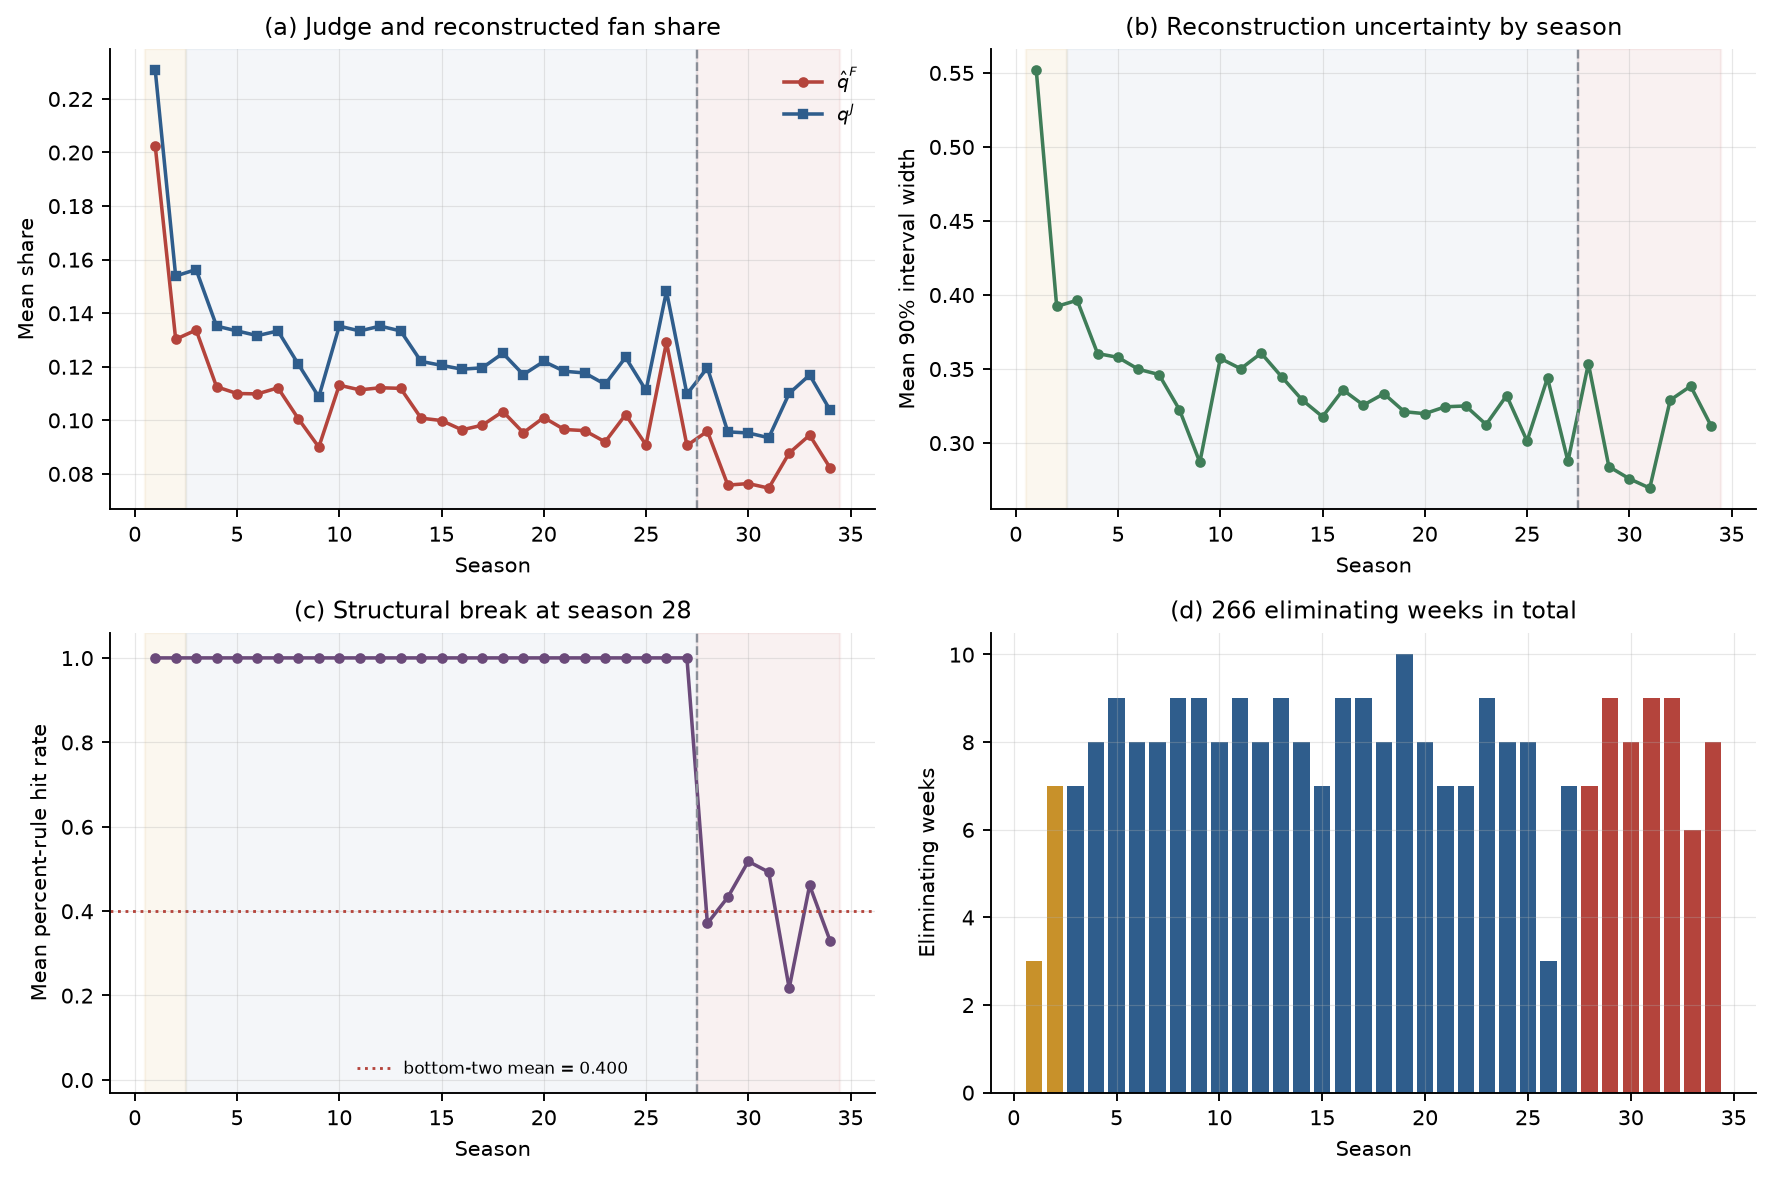
\includegraphics[width=0.94\textwidth]{figures_ext/fig03_season_dynamics.png}
\caption{Season-level dynamics. (a) Mean judge share and mean reconstructed fan share.
(b) Mean $90\%$ credible-interval width. (c) Mean percent-rule hit rate over eliminating
weeks; the dashed line marks the $0.400$ bottom-two average. (d) Number of eliminating weeks
per season ($266$ in total). Shaded bands mark the three fusion regimes.}
\label{fig:seasondyn}
\end{figure}

Panel~(c) is the sharpest descriptive result: the hit rate is exactly $1.000$ in every season
from $1$ through $27$ and drops abruptly to between $0.37$ and $0.43$ from season $28$ onward.
There is no gradual drift. Panel~(d) confirms that this is not a sample-size artefact --- the
late seasons actually contribute \emph{more} eliminating weeks than the early ones. A complete
season-by-season breakdown including couple--weeks, mean shares, mean interval width and worst
split-$\hat R$ is given in Table~\ref{tab:seasonstats}.

\subsection{The Structure of Uncertainty}\label{sec:uncertainty}

The problem asks explicitly whether the certainty of the estimated fan vote is always the
same. It is not, but the \emph{direction} of the heterogeneity is subtler than a first reading
suggests, and it depends on whether width is measured in absolute or field-size-normalised
terms.

Across all $2{,}777$ couple--weeks the $90\%$ interval width $\Delta$ has mean $0.328$,
median $0.313$, $5$th percentile $0.065$ and $95$th percentile $0.607$, with a full range of
$0.022$ to $0.898$. The posterior standard deviation has mean $0.088$. Regressing (in the
sense of raw correlation) $\Delta$ on the weekly design variables gives
$r=-0.649$ against the number of surviving couples, $r=+0.563$ against competition week,
$r=-0.427$ against the number of active constraints, and $r=+0.143$ against the within-week
standard deviation of judge shares. In \emph{absolute} terms, therefore, the widest intervals
occur late in the season in small fields, where each surviving couple commands a large share
and the simplex face is wide. This is the opposite of the naive expectation that large fields
are harder to identify.

That apparent paradox is a scale effect. Rescaling by field size,
$\Delta^{\rm rel}=n_{sw}\Delta$ (mean $2.833$), reverses two of the signs:
$r=+0.261$ against field size and $r=-0.241$ against week. On a comparable scale, large
early-season fields \emph{are} the least identified, exactly as the intuition predicts.
Figure~\ref{fig:uncstruct} shows both measures side by side, and
Tables~\ref{tab:uncertaintyweeks} and~\ref{tab:judgebaseline} give the week-by-week and
field-size breakdowns. We therefore recommend that any operational use of these estimates
report $\Delta^{\rm rel}$ alongside $\Delta$; the absolute width alone can be misleading.

\begin{figure}[H]
\centering
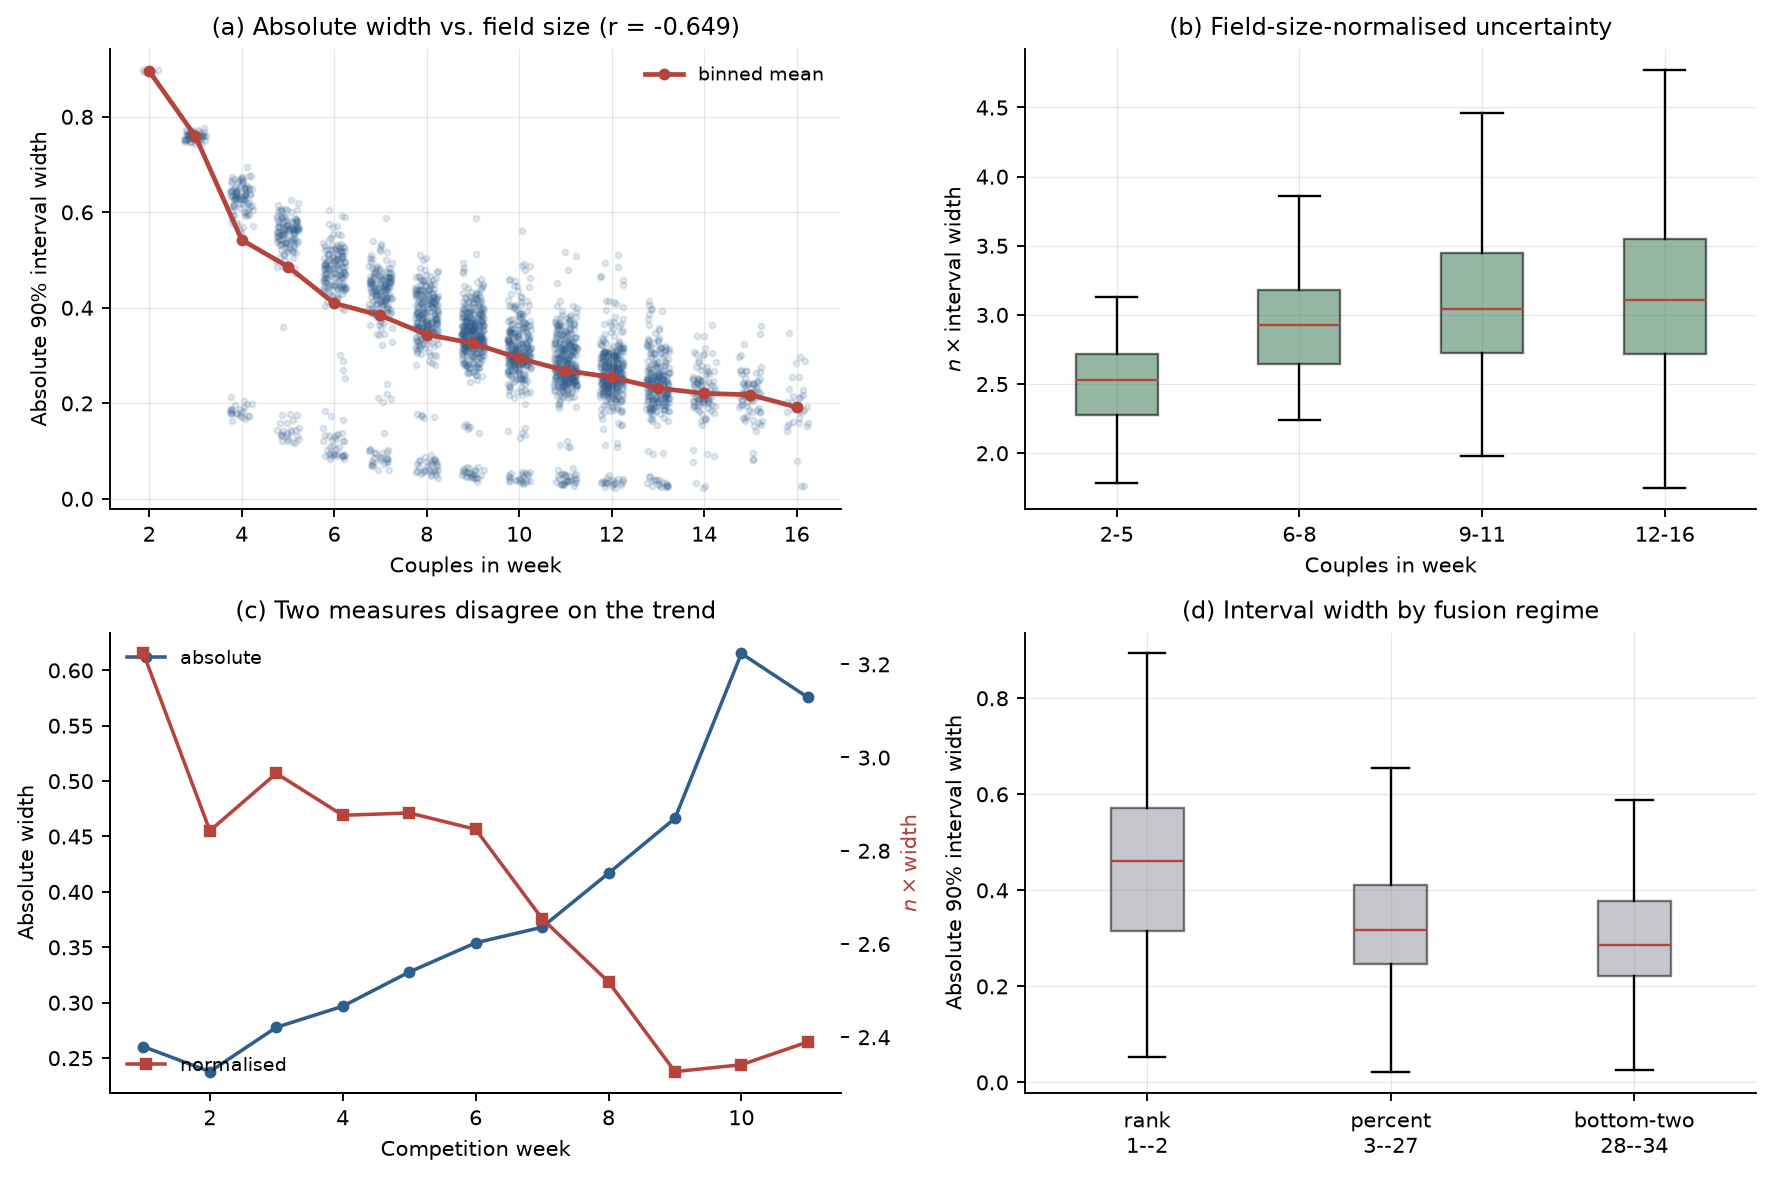
\includegraphics[width=0.94\textwidth]{figures_ext/fig04_uncertainty_structure.png}
\caption{What drives reconstruction uncertainty. (a) Absolute interval width against field
size with binned means. (b) Field-size-normalised width by field-size stratum. (c) Absolute
(left axis) and normalised (right axis) width by competition week --- the two trend in opposite
directions. (d) Absolute width by fusion regime.}
\label{fig:uncstruct}
\end{figure}

% AUTO-GENERATED table — values computed by analyze_extended.py
\begin{table}[H]
\centering
\caption{Uncertainty by competition week. $\overline{\Delta}$ is the mean absolute $90\%$ credible-interval width; $\overline{\Delta}_{\rm rel}=n\,\overline{\Delta}$ rescales it by the field size so that intervals are comparable across weeks with different numbers of surviving couples. Absolute width grows late in a season because shares themselves grow; the rescaled width is the comparable measure.}
\label{tab:uncertaintyweeks}
\begin{tabular}{lrrrrr}
\toprule
Week & $n$ & Couples & $\overline{q^F}$ & $\overline{\Delta}$ & $\overline{\Delta}_{\rm rel}$ \\ 
\midrule
1 & 421 & 12.6 & 0.061 & 0.260 & 3.22 \\ 
2 & 404 & 12.2 & 0.067 & 0.238 & 2.84 \\ 
3 & 360 & 10.9 & 0.075 & 0.278 & 2.97 \\ 
4 & 326 & 10.0 & 0.084 & 0.297 & 2.88 \\ 
5 & 288 & 9.0 & 0.092 & 0.328 & 2.88 \\ 
6 & 261 & 8.3 & 0.103 & 0.354 & 2.85 \\ 
7 & 228 & 7.3 & 0.117 & 0.368 & 2.65 \\ 
8 & 191 & 6.2 & 0.143 & 0.417 & 2.52 \\ 
9 & 152 & 5.1 & 0.179 & 0.466 & 2.33 \\ 
10 & 109 & 4.0 & 0.238 & 0.615 & 2.34 \\ 
11 & 37 & 4.2 & 0.214 & 0.576 & 2.39 \\ 
\bottomrule
\end{tabular}
\end{table}


\subsection{Judge--Fan Disagreement in the Fine Ordering}

Figure~\ref{fig:channels} decomposes the $0.832$ level correlation and $0.153$ rank-vector
correlation into interpretable quantities. Panel~(a) plots $q^J$ against $\tilde q^F$; the
cloud follows the diagonal but with substantial scatter. Panel~(b) plots the within-week
reallocation $\tilde q^F-q^J$, which has mean zero \emph{by construction} (both vectors sum to
one within a week) but standard deviation $0.040$, with $5$th and $95$th percentiles of
$-0.080$ and $+0.057$. The dispersion is largest in the rank era ($0.060$), intermediate in
the percent era ($0.044$) and smallest in the bottom-two era ($0.024$) --- evidence that the
later rules compress the scope for fan-driven reallocation.

Panel~(c) is the more telling diagnostic: the absolute difference $|r^F-r^J|$ has mean
$3.27$ rank positions, median $2.5$, $90$th percentile $7$, and exceeds one position in
$65.8\%$ of all couple--weeks. In other words, for roughly two thirds of couple--weeks the
audience and the panel place the couple at least two ordinal positions apart. This is the
mechanical source of rule sensitivity: rank fusion is a function of these disagreeing ordinal
vectors, while percent fusion is a function of the largely agreeing share levels.

\begin{figure}[H]
\centering
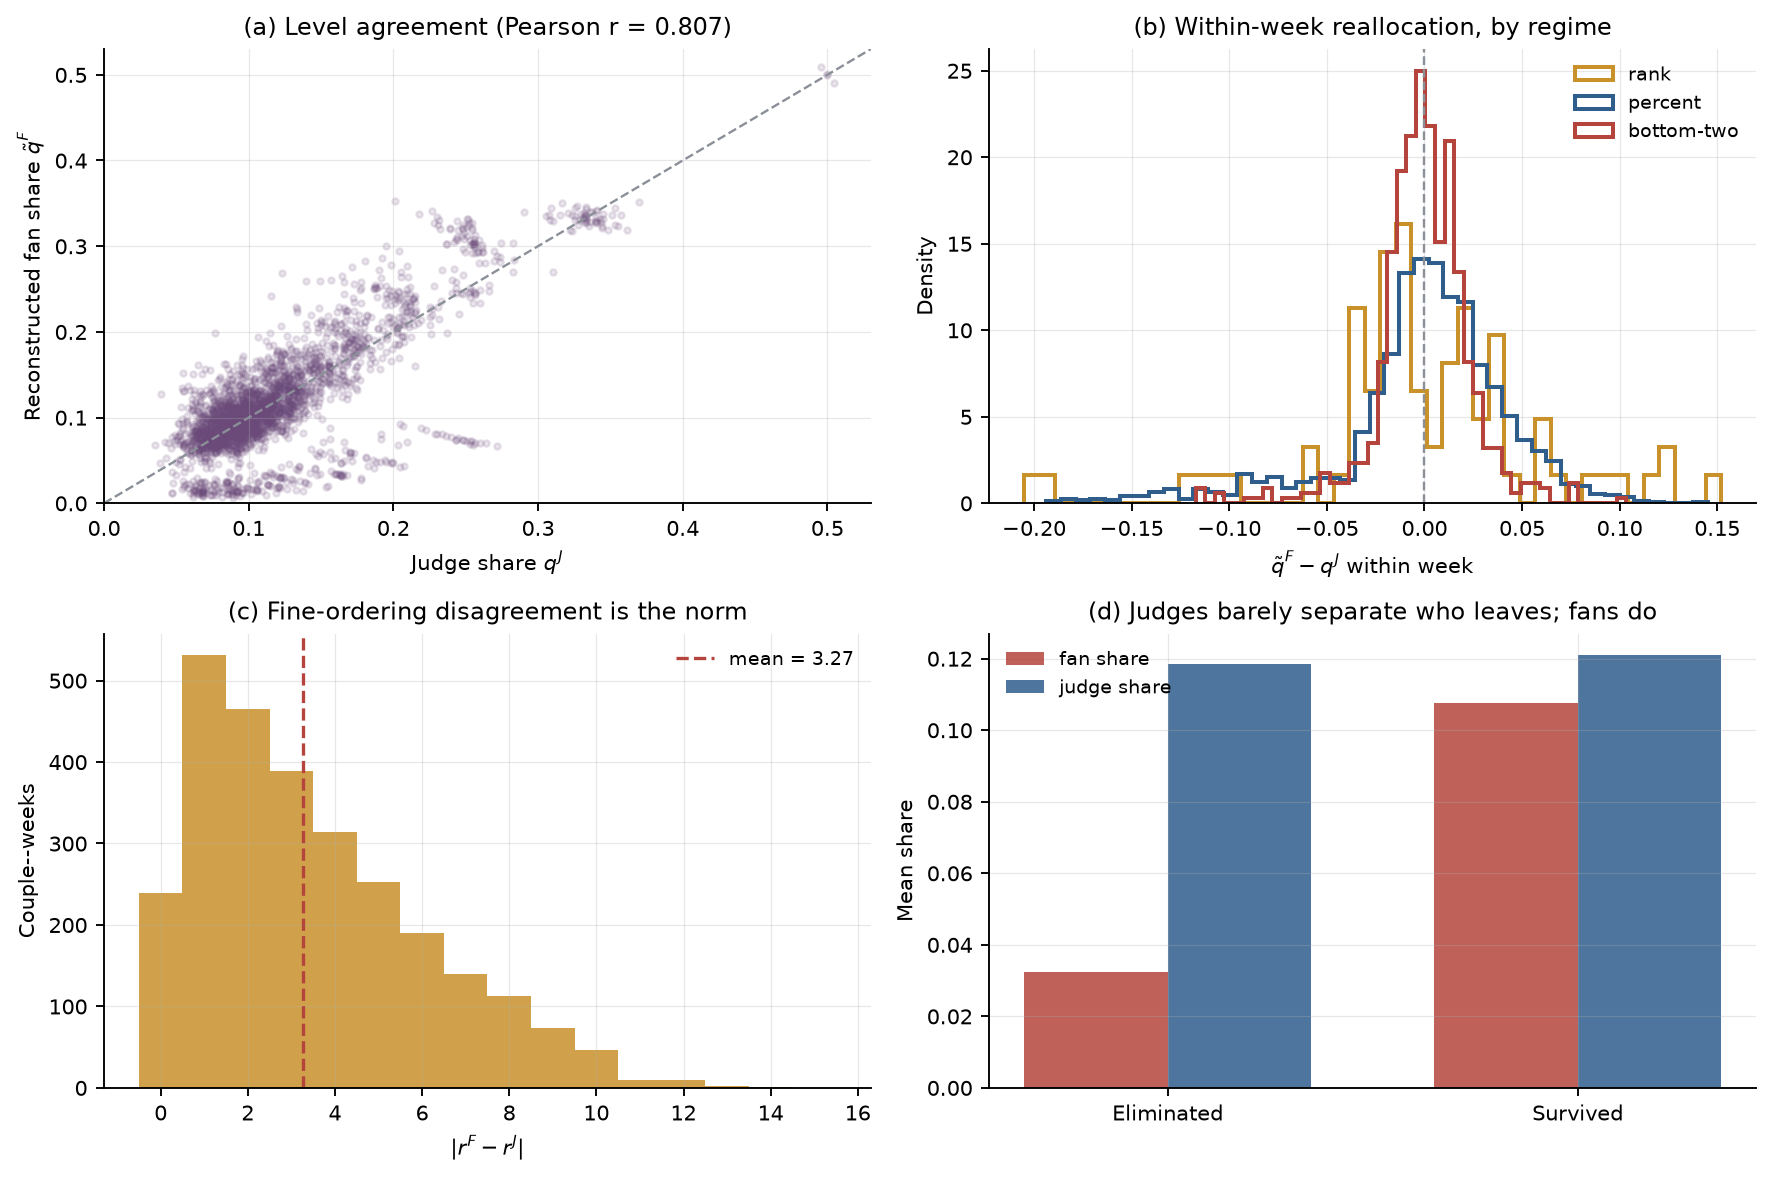
\includegraphics[width=0.94\textwidth]{figures_ext/fig05_judge_fan_channels.png}
\caption{Judge and fan channels. (a) Judge share versus renormalised fan share, with the
identity line. (b) Within-week reallocation $\tilde q^F-q^J$ by fusion regime. (c) Absolute
rank displacement $|r^F-r^J|$. (d) Mean share levels for eliminated versus surviving couples.}
\label{fig:channels}
\end{figure}

Panel~(d) contains a result that is easy to overlook. Eliminated couples have mean fan share
$0.032$ against $0.108$ for survivors --- a $3.3$-fold separation --- but mean judge shares of
$0.118$ and $0.121$, essentially \emph{identical}. Their mean interval width is also far
narrower ($0.091$ versus $0.358$) because the elimination constraint pins the eliminated
couple near the bottom of the polytope. Thus the judge channel alone barely distinguishes who
goes home, while the reconstructed fan channel does. We stress that the latter separation is
partly structural (the polytope enforces it); the next subsection therefore isolates a
\emph{non-circular} benchmark.

\subsection{A Non-Circular Benchmark: the Judge-Only Baseline}\label{sec:judgebaseline}

Because Model~1's feasible polytope is constructed to contain the observed elimination, its
near-perfect hit rate in seasons 1--27 cannot be read as predictive accuracy. A clean,
non-circular benchmark is available without any reconstructed quantity at all: in each
eliminating week, ask whether the couple with the \emph{lowest judge share} is the one actually
eliminated. This uses only the official scores.

The answer is $\mathbf{0.444}$ pooled over all $266$ eliminating weeks. Stratifying by regime
gives $0.400$ in the rank era ($10$ weeks), $0.460$ in the percent era ($200$ weeks) and
$0.393$ in the bottom-two era ($56$ weeks). Equivalently, the eliminated couple holds the
worst judge rank in only $42.2\%$ of eliminations and sits at mean normalised judge rank
$0.781$ (where $1$ denotes the worst). Judge scores alone therefore fail to identify the
elimination in a clear majority of weeks, in \emph{every} regime. This is the cleanest
model-free evidence that a second channel --- the audience vote, and in later seasons the
judge save --- is necessary to explain outcomes.

\begin{figure}[H]
\centering
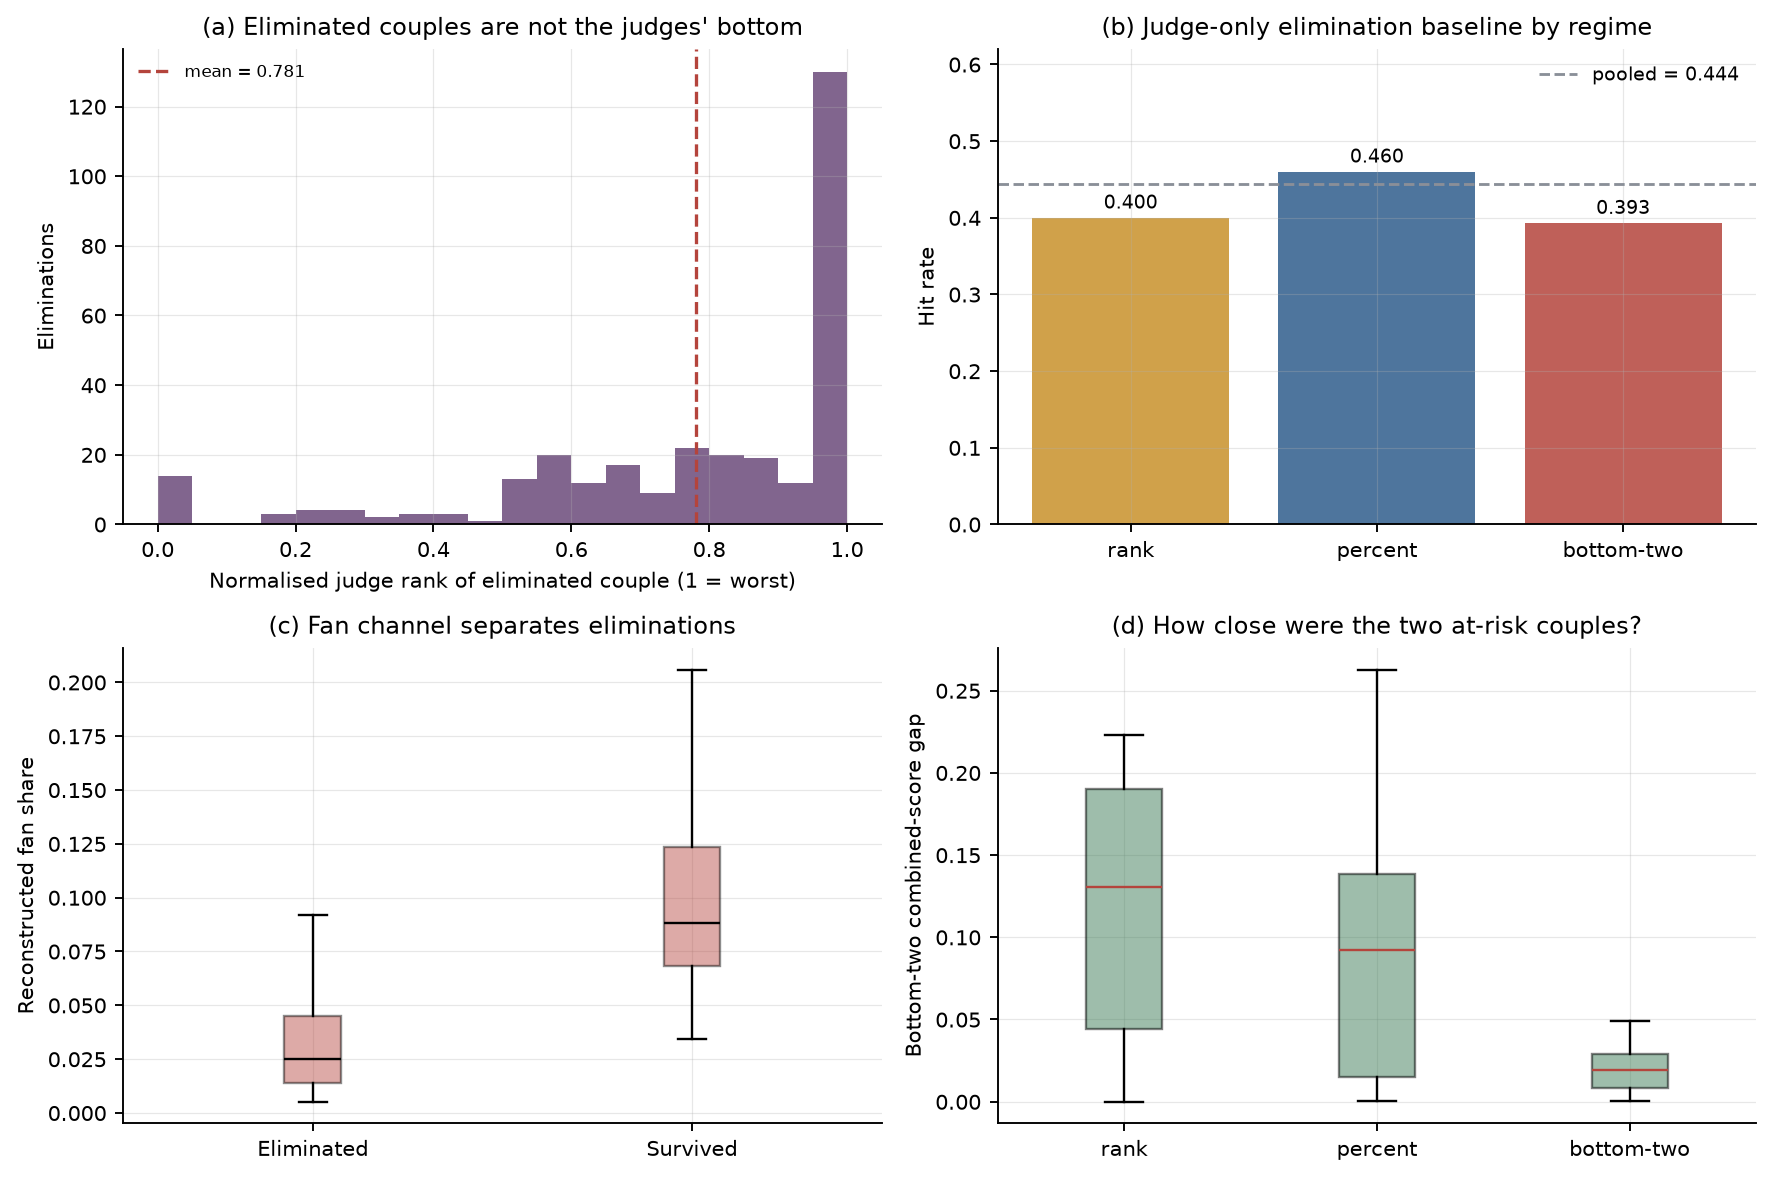
\includegraphics[width=0.94\textwidth]{figures_ext/fig06_elimination_evidence.png}
\caption{Non-circular elimination evidence. (a) Normalised judge rank of eliminated couples.
(b) Judge-only hit rate by regime, with the pooled $0.444$ line. (c) Reconstructed fan share
for eliminated versus surviving couples. (d) Gap between the two lowest combined scores by
regime (bottom-two margin distribution).}
\label{fig:elimevidence}
\end{figure}

% AUTO-GENERATED table — values computed by analyze_extended.py
\begin{table}[H]
\centering
\caption{Uncertainty by field size, and the judge-only elimination baseline. ``Judge-only hit'' is the fraction of eliminating weeks in which the couple with the lowest judge share is the one actually eliminated --- a non-circular benchmark because it uses no reconstructed fan share.}
\label{tab:judgebaseline}
\begin{tabular}{lrrrr}
\toprule
Stratum & $n$ & $\overline{\Delta}$ & $\overline{\Delta}_{\rm rel}$ & Judge-only hit \\ 
\midrule
\multicolumn{5}{l}{\emph{Field size}} \\ 
2-5 couples & 322 & 0.559 & 2.30 & -- \\ 
6-8 couples & 654 & 0.374 & 2.65 & -- \\ 
9-11 couples & 1001 & 0.297 & 2.94 & -- \\ 
12-16 couples & 800 & 0.237 & 3.06 & -- \\ 
\midrule
\multicolumn{5}{l}{\emph{Fusion regime}} \\ 
rank & 10 & -- & -- & 0.400 \\ 
percent & 200 & -- & -- & 0.460 \\ 
bottom-two & 56 & -- & -- & 0.393 \\ 
\bottomrule
\end{tabular}
\end{table}


Figure~\ref{fig:elimevidence}(d) adds a useful qualification: the gap between the two lowest
percent-combined scores is small in the bottom-two regime, so the judge save typically decides
between genuinely close couples. This is consistent with interpreting the save as a
\emph{bounded} merit safeguard rather than an arbitrary override, and it qualifies the
stronger claim one might otherwise draw from the $0.400$ hit rate.

\subsection{Trajectories of the Four Named Controversies}\label{sec:trajectories}

Table~\ref{tab:controversy} reports final-week quantities for the four contestants named in the
problem. Figure~\ref{fig:trajectories} shows their full week-by-week paths, which reveal how
those final values arose. All four carry a persistent fan premium: $\tilde q^F$ exceeds $q^J$
in $6$ of $8$ weeks for Jerry Rice, $7$ of $8$ for Billy Ray Cyrus, $9$ of $10$ for Bristol
Palin and $8$ of $9$ for Bobby Bones. Their mean judge ranks over those runs are $4.69$,
$6.88$, $6.00$ and $7.22$ respectively --- Palin and Bones spent most of their seasons in the
bottom half of the judges' ordering while retaining above-average audience support.

\begin{figure}[H]
\centering
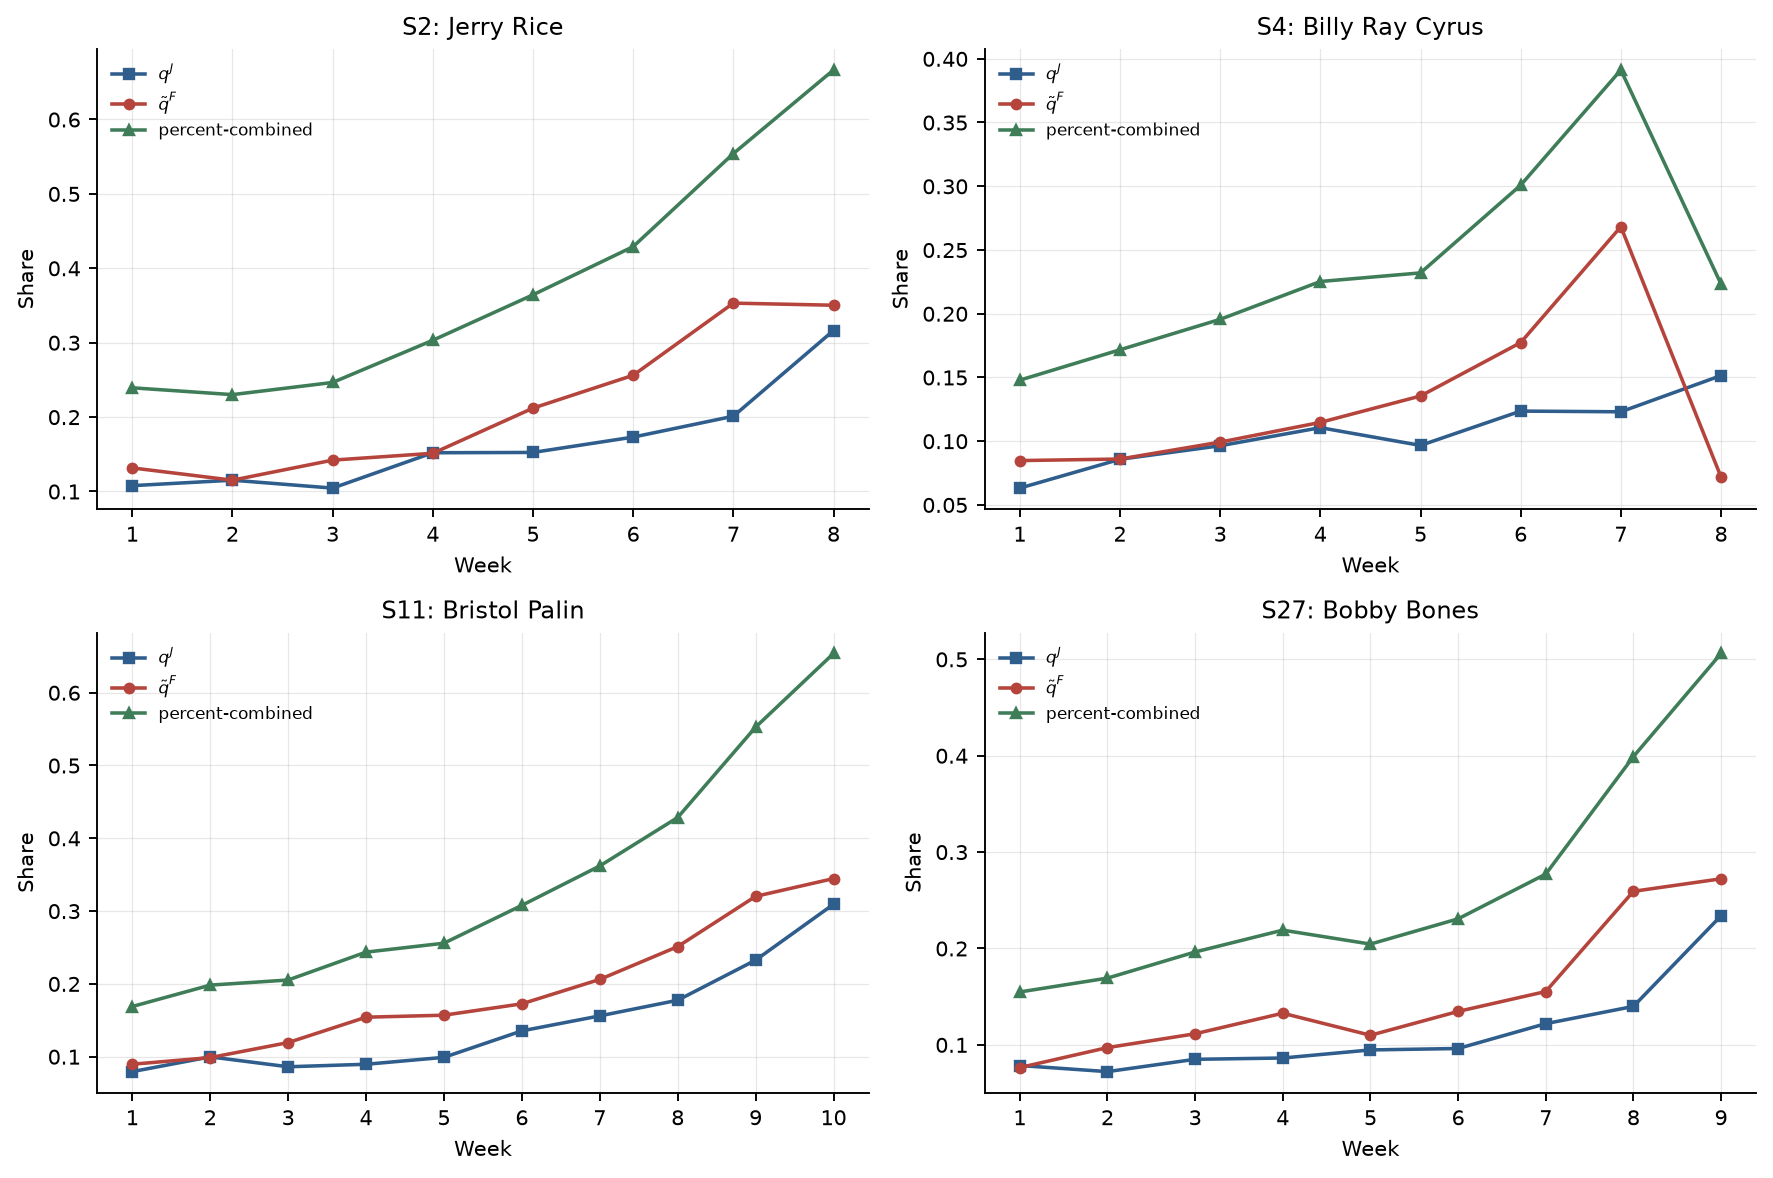
\includegraphics[width=0.94\textwidth]{figures_ext/fig11_controversy_trajectories.png}
\caption{Weekly trajectories of the four named controversy contestants. Blue squares: judge
share $q^J$; red circles: renormalised reconstructed fan share $\tilde q^F$; green triangles:
percent-combined score. The persistent red-above-blue gap is the signature of a fan-driven
survival, not a single-week anomaly.}
\label{fig:trajectories}
\end{figure}

Mean renormalised fan shares are $0.214$ (Rice), $0.130$ (Cyrus), $0.191$ (Palin) and $0.150$
(Bones), against mean judge shares of $0.165$, $0.106$, $0.146$ and $0.112$. Cyrus is the
outlier: his fan premium is positive but small, which is why rank fusion does not rescue him
whereas it does rescue the other three. The trajectories therefore corroborate, with
season-long rather than final-week evidence, the conclusion of Section~\ref{sec:results}.

\subsection{Covariate Channels and Casting Effects}\label{sec:covariates}

Model~3 decomposes the two channels by celebrity covariates. Figure~\ref{fig:covariates} and
Table~\ref{tab:covariates} extend that analysis with age bands, industry groups and
professional-partner effects. Age is negatively associated with \emph{both} channels
(Pearson $r=-0.166$ for fan share, $-0.244$ for judge share), so the fan-specific age penalty
is smaller than the raw fan--age correlation suggests: the judge channel declines at least as
steeply. The binned mean fan share is $0.108$ for ages $\le 26$, $0.109$ for $27$--$34$,
$0.097$ for $35$--$43$ and $0.082$ above $43$ --- a $24\%$ decline from the youngest to the
oldest quartile, with a mild non-monotone peak in the $27$--$34$ band.

Industry gaps are modest: athletes lead at $0.106$, actors and singers are near $0.100$,
television/media at $0.094$, and models trail at $0.076$. The fan--judge gap $\Delta$ is
negative for every industry group because judge shares are uniformly higher in this panel,
but its \emph{variation} across groups is small. The largest covariate effect we observe is
the professional partner: $0.120$ for Julianne Hough and $0.117$ for Derek Hough at the top
against $0.066$ for Brandon Armstrong and $0.064$ for Britt Stewart at the bottom, a ratio
close to $1.9$. Home-country status is essentially uninformative ($0.0994$ for US-based versus
$0.0986$ for non-US contestants). These magnitudes justify the paper's conclusion that
demographics are secondary to dance quality and partner effects.

\begin{figure}[H]
\centering
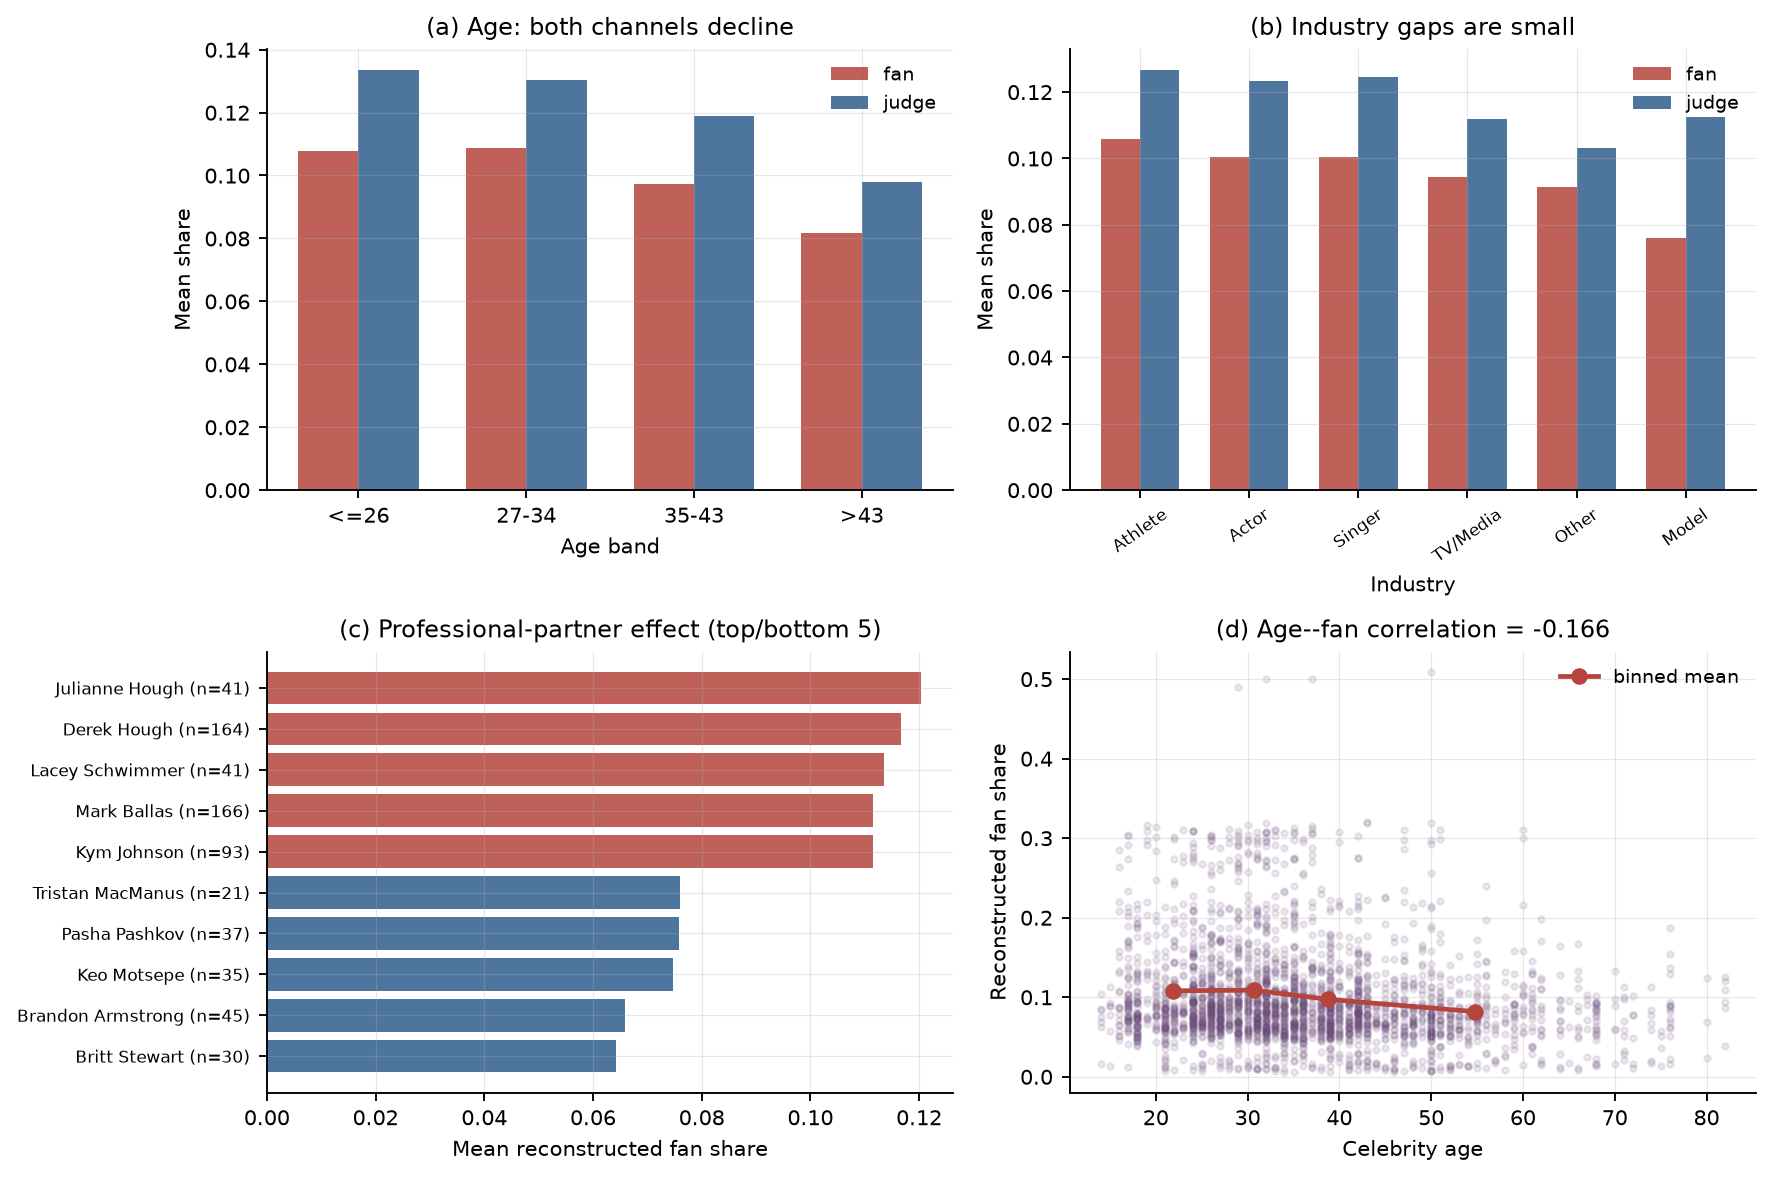
\includegraphics[width=0.94\textwidth]{figures_ext/fig12_covariate_channels.png}
\caption{Covariate channel comparison. (a) Fan and judge mean shares by age band.
(b) By industry group (groups with at least 25 couple--weeks). (c) Mean reconstructed fan
share for the five highest and five lowest professional partners with at least 20 couple--weeks.
(d) Age versus fan share with binned means.}
\label{fig:covariates}
\end{figure}

% AUTO-GENERATED table — values computed by analyze_extended.py
\begin{table}[H]
\centering
\caption{Covariate channel comparison (Model 3 panel). Mean reconstructed fan share and judge share by celebrity age band and by industry group (groups with at least 25 couple--weeks). $\Delta=\overline{q^F}-\overline{q^J}$ isolates the fan-specific premium.}
\label{tab:covariates}
\begin{tabular}{lrrrr}
\toprule
Group & $n$ & $\overline{q^F}$ & $\overline{q^J}$ & $\Delta$ \\ 
\midrule
\multicolumn{5}{l}{\emph{Age band}} \\ 
<=26 & 670 & 0.108 & 0.134 & -0.026 \\ 
27-34 & 755 & 0.109 & 0.130 & -0.022 \\ 
35-43 & 697 & 0.097 & 0.119 & -0.022 \\ 
>43 & 655 & 0.082 & 0.098 & -0.016 \\ 
\midrule
\multicolumn{5}{l}{\emph{Industry}} \\ 
Athlete & 658 & 0.106 & 0.127 & -0.021 \\ 
Actor & 882 & 0.100 & 0.123 & -0.023 \\ 
Singer & 414 & 0.100 & 0.125 & -0.024 \\ 
TV/Media & 660 & 0.094 & 0.112 & -0.017 \\ 
Other & 87 & 0.091 & 0.103 & -0.012 \\ 
Model & 76 & 0.076 & 0.112 & -0.036 \\ 
\bottomrule
\end{tabular}
\end{table}


\subsection{Regime-Level Summary}\label{sec:regimesummary}

Table~\ref{tab:erastats} consolidates the three regimes. The transition from $210$
non-bottom-two eliminating weeks (mean hit rate $1.000$, mean Brier $0.007$) to $56$
bottom-two weeks (mean hit rate $0.400$, mean Brier $0.547$) is a $0.593$ absolute drop in
hit rate and an almost eighty-fold increase in Brier score, while mean credible-interval width
barely moves ($0.332$ to $0.306$). The failure is therefore attributable to the \emph{rule},
not to a deterioration in the quality of the reconstruction. This distinction is essential to
the interpretation offered in Section~\ref{sec:discussion}.

% AUTO-GENERATED table — values computed by analyze_extended.py
\begin{table}[H]
\centering
\caption{Regime comparison. Hit rate and $\kappa$ are averaged over eliminating weeks; credible-interval width is averaged over all couple--weeks in the regime.}
\label{tab:erastats}
\begin{tabular}{lrrrrrr}
\toprule
Regime & C--W & Weeks & Elim. & Hit rate & $\overline{\Delta}$ & Brier \\ 
\midrule
rank & 78 & 14 & 10 & 1.000 & 0.446 & 0.000 \\ 
percent & 1997 & 248 & 200 & 1.000 & 0.332 & 0.007 \\ 
bottom-two & 702 & 73 & 56 & 0.400 & 0.306 & 0.547 \\ 
\bottomrule
\end{tabular}
\end{table}


%=====================================================================


%=====================================================================
\section{Counterfactual Fusion Design and the Rule--Outcome Frontier}\label{sec:counterfactual}
%=====================================================================

The problem asks not only to estimate the hidden vote but to advise the producers on the
fusion rule. To move from a handful of named controversies to a systematic comparison, we
replay three decades of eliminations under a continuous family of rules and measure how often
each rule reproduces the observed outcome. This section states the replay design, reports the
resulting frontier, and --- importantly --- delimits what the exercise can and cannot prove.

\subsection{Replay Design}\label{sec:replaydesign}

For a fixed weight $w\in[0,1]$ we form the counterfactual combined score

\begin{equation}
\label{eq:weightedscore}
  C_{i,sw}(w) \;=\; w\,q^J_{i,sw} \;+\; (1-w)\,\tilde q^F_{i,sw},
  \qquad i\in S_{sw},
\end{equation}

and predict that the couple minimising $C_{i,sw}(w)$ is eliminated. The endpoints are
informative: $w=1$ is a judge-only rule using official scores exclusively, while $w=0$ is a
fan-only rule. The historical percent rule corresponds to $w=0.5$ up to the renorm\-alisation
used here. An ordinal analogue replaces both shares by their within-week ranks,

\begin{equation}
\label{eq:weightedrank}
  C^{\rm rank}_{i,sw}(w) \;=\; w\,r^J_{i,sw} \;+\; (1-w)\,r^F_{i,sw},
\end{equation}

with the couple \emph{maximising} $C^{\rm rank}$ eliminated, since rank $1$ denotes the best
couple. We scan $w$ on a grid of $21$ points and compute, for each, the fraction of the $266$
eliminating weeks in which the predicted and observed eliminations coincide. All shares are
within-week renormalised so that the two channels enter on the same scale
(Section~\ref{sec:eda_source}).

\paragraph{A necessary caveat on circularity.} The reconstructed fan share is drawn from a
polytope whose inequalities \emph{enforce the observed elimination}. Consequently, for any
$w$ that gives the fan channel appreciable weight, a high consistency rate is a designed
property of the reconstruction, not out-of-sample predictive accuracy. We therefore shade the
region $w\lesssim0.55$ in Figure~\ref{fig:frontier} and refrain from interpreting it as model
validation. Exactly one point on the curve is free of this circularity: at $w=1$ the score
contains no reconstructed quantity at all, and the resulting $0.444$ is the judge-only
benchmark of Section~\ref{sec:judgebaseline}. The legitimate reading of the frontier is thus
about \emph{sensitivity} --- how quickly consistency degrades as the audience channel is
removed --- not about forecast skill. A genuine out-of-sample test would require the Model~2
generative likelihood discussed in Section~\ref{sec:m2_status}.

\begin{figure}[H]
\centering
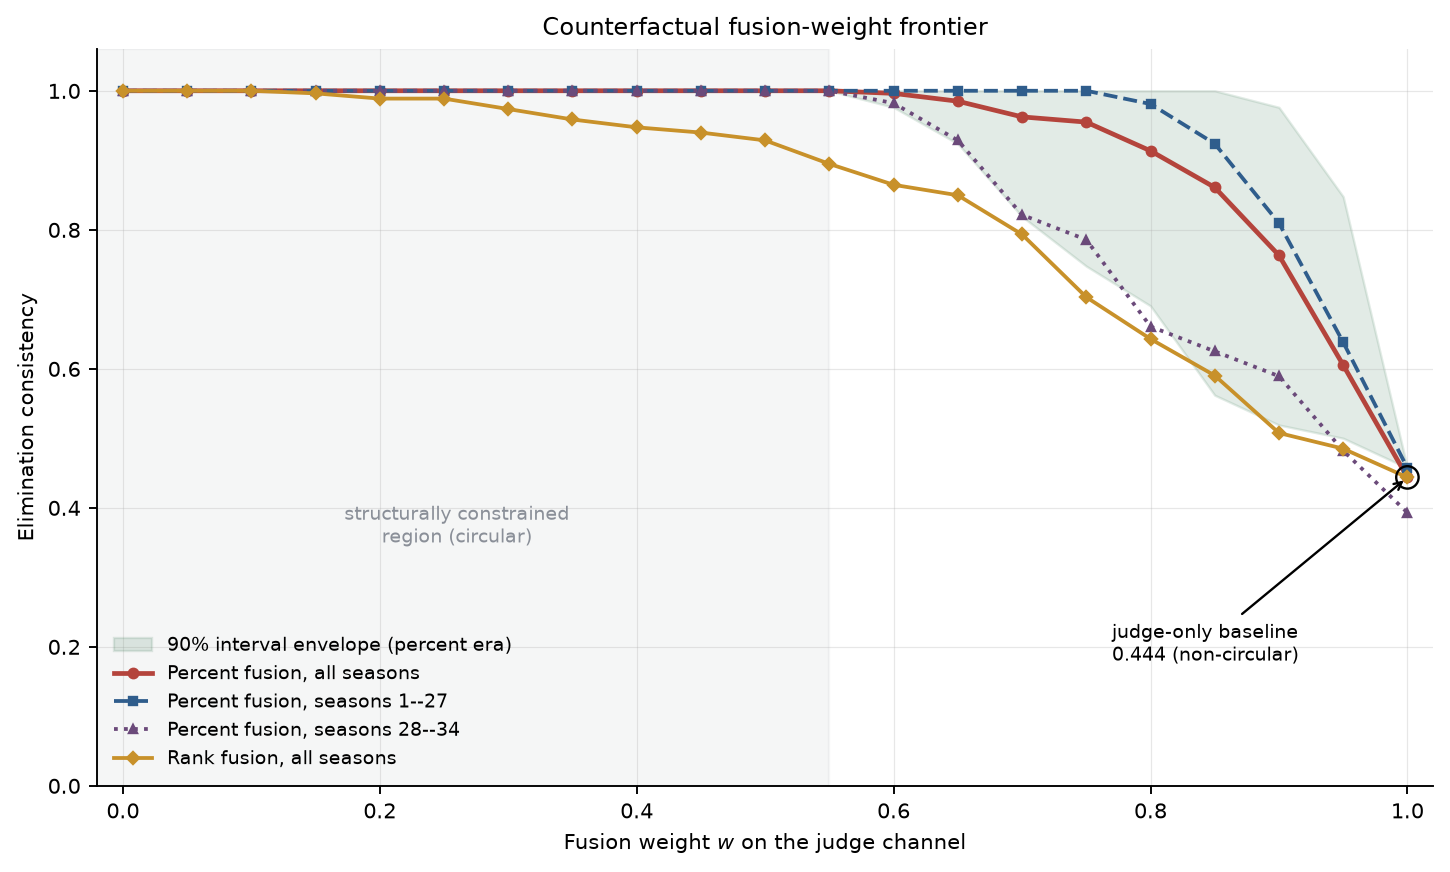
\includegraphics[width=0.88\textwidth]{figures_ext/fig07_fusion_weight_frontier.png}
\caption{Counterfactual fusion-weight frontier. Elimination consistency as the weight $w$ on
the judge channel varies from $0$ (fan-only) to $1$ (judge-only). The shaded left region is
structurally constrained and must not be read as predictive accuracy. The green envelope shows
the range obtained by replacing the posterior median with the $5\%$ and $95\%$ fan-share bounds.
The circled point is the non-circular judge-only baseline.}
\label{fig:frontier}
\end{figure}

\subsection{The Frontier and What It Shows}

Table~\ref{tab:weights} reports the full grid. Three features stand out.

\emph{(i) The judge channel alone is insufficient.} At $w=1$ consistency is $0.444$ pooled,
$0.457$ in seasons 1--27 and $0.393$ in seasons 28--34. No amount of reweighting can make a
judge-only rule reproduce more than about half of the observed eliminations. This is the
model-free anchor of the whole analysis.

\emph{(ii) Consistency degrades smoothly, not abruptly, and later seasons degrade faster.} At
$w=0.75$ the pooled rate is $0.955$, but the percent era remains at $1.000$ while the
bottom-two era has already fallen to $0.786$; at $w=0.8$ the split widens to $0.981$ versus
$0.661$. The late seasons are more sensitive to the removal of audience weight because the
judge save introduces a second, judge-driven decision that the combined score cannot express.
This is a quantitative complement to the $0.400$ hit-rate finding.

\emph{(iii) Rank fusion is more weight-sensitive than percent fusion.} The ordinal curve falls
to $0.929$ at $w=0.5$, $0.865$ at $w=0.6$, $0.703$ at $w=0.75$ and $0.508$ at $w=0.9$,
whereas the percent curve stays above $0.96$ until $w=0.7$. Ordinal ranks are coarse (only
$n_{sw}$ distinct values) and ties are frequent, so small changes in $w$ can reorder two
near-equal couples. This is the same mechanism that makes rank fusion favour fan favourites:
it discards the magnitude of a judge advantage that percent fusion would preserve.

% AUTO-GENERATED table — values computed by analyze_extended.py
\begin{table}[H]
\centering
\caption{Counterfactual elimination consistency as the fusion weight $w$ on the judge channel varies. Score $=w\,q^J+(1-w)\,\hat q^F$; the predicted elimination is the couple minimising the score. Percent-era = seasons 1--27, bottom-two era = seasons 28--34. The rank column uses $w\,r^J+(1-w)\,r^F$ on ordinal ranks.}
\label{tab:weights}
\begin{tabular}{lcccc}
\toprule
$w$ (judge weight) & All seasons & Percent era & Bottom-two era & Rank fusion \\ 
\midrule
0.0 & 1.000 & 1.000 & 1.000 & 1.000 \\ 
0.1 & 1.000 & 1.000 & 1.000 & 1.000 \\ 
0.2 & 1.000 & 1.000 & 1.000 & 0.989 \\ 
0.3 & 1.000 & 1.000 & 1.000 & 0.974 \\ 
0.4 & 1.000 & 1.000 & 1.000 & 0.947 \\ 
0.5 & 1.000 & 1.000 & 1.000 & 0.929 \\ 
0.6 & 0.996 & 1.000 & 0.982 & 0.865 \\ 
0.7 & 0.962 & 1.000 & 0.821 & 0.793 \\ 
0.8 & 0.913 & 0.981 & 0.661 & 0.643 \\ 
0.9 & 0.763 & 0.809 & 0.589 & 0.507 \\ 
1.0 & 0.444 & 0.457 & 0.393 & 0.444 \\ 
\bottomrule
\end{tabular}
\end{table}


\subsection{Uncertainty-Aware Replay}\label{sec:intervalreplay}

Because the posterior median is only one point in a wide feasible set, a replay that uses it
alone overstates what is identified. We therefore repeat the percent-era scan three times,
substituting the $5\%$ lower bound $\hat q^F_{5}$, the median, and the $95\%$ upper bound
$\hat q^F_{95}$ for the fan channel. Figure~\ref{fig:intervalreplay} shows the resulting
envelope. For $w\le0.5$ all three curves agree at $1.000$, so conclusions in the
historically relevant range are interval-robust. At $w=0.75$ the lower-bound replay falls to
$0.748$ while the upper bound stays at $1.000$; at $w=0.9$ the spread is $0.519$ to $0.976$.
Any claim about high-weight rules is therefore sensitive to where in the credible set the true
vote lies, and should be reported with this envelope rather than as a single number.

\begin{figure}[H]
\centering
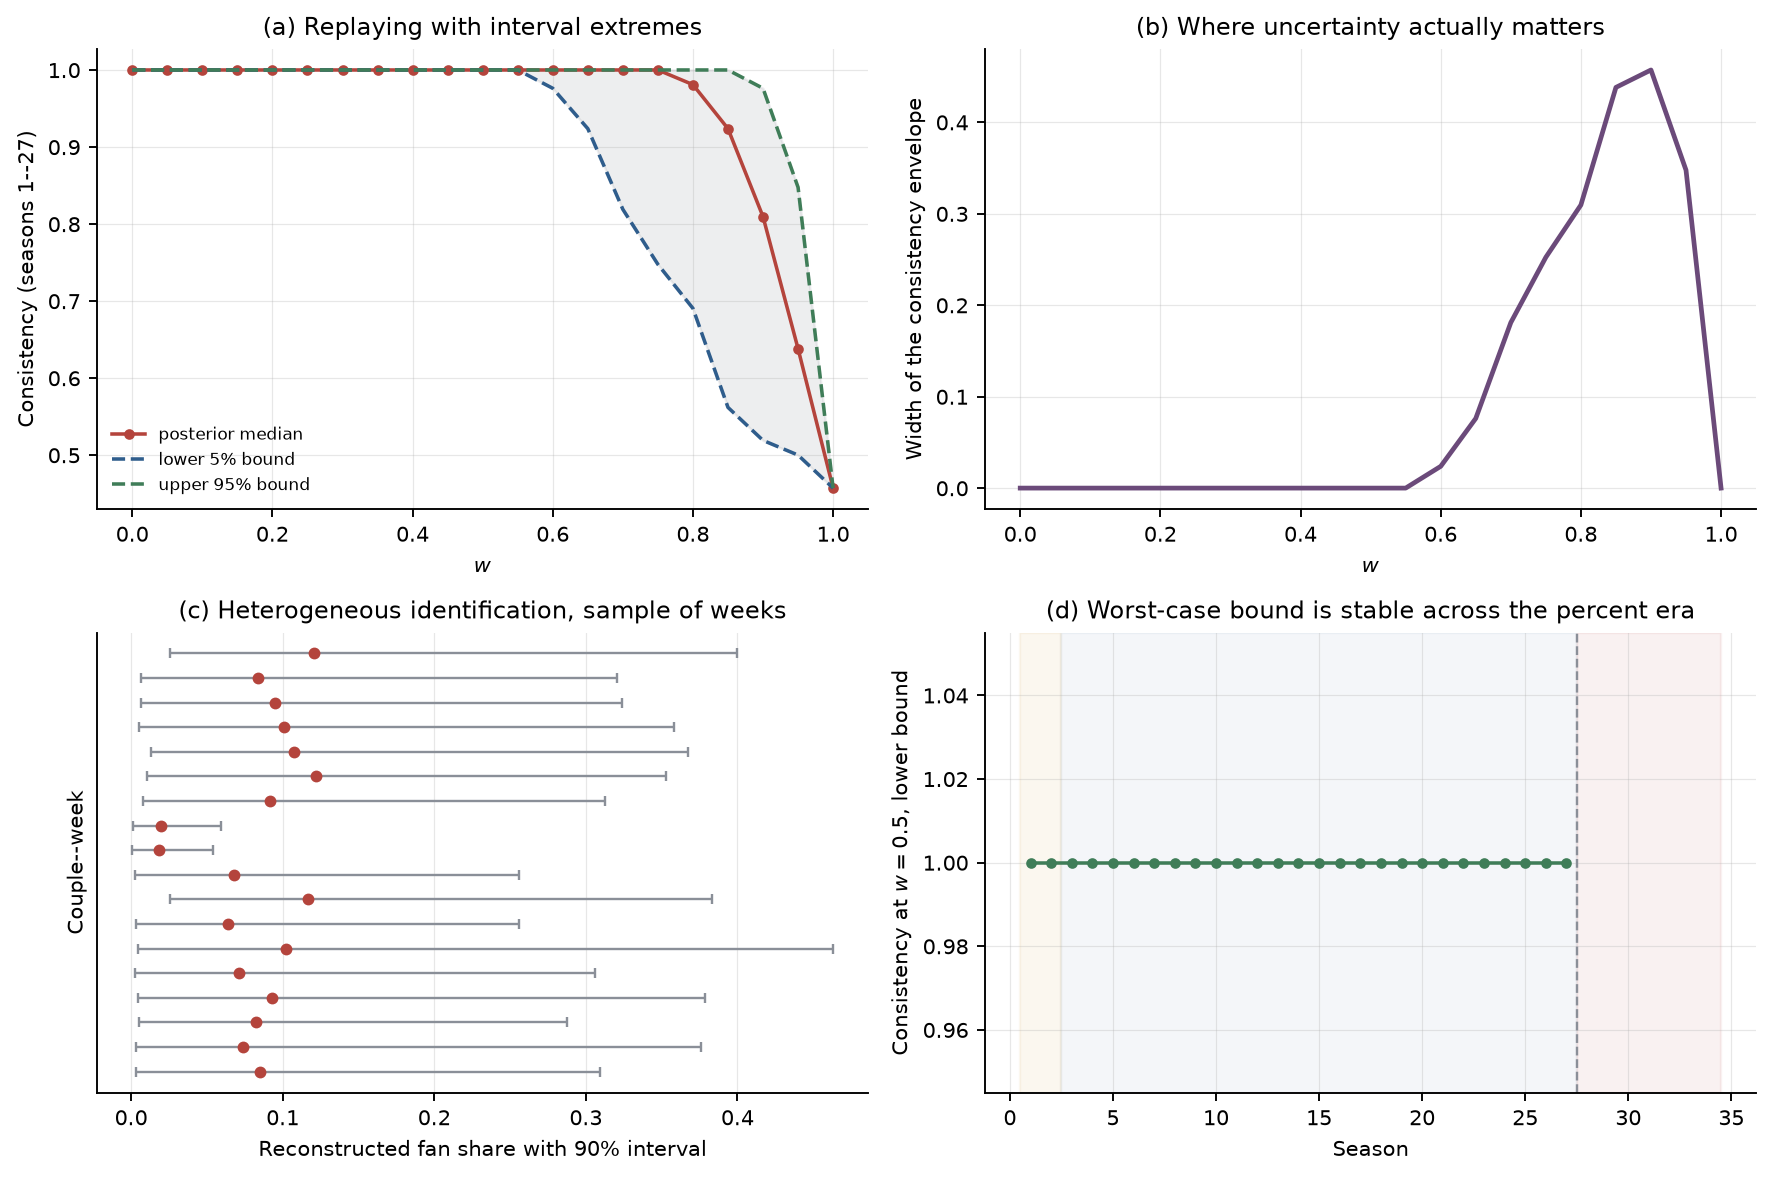
\includegraphics[width=0.94\textwidth]{figures_ext/fig13_interval_robust_replay.png}
\caption{Uncertainty-aware counterfactual replay. (a) Consistency under the median, $5\%$ and
$95\%$ fan-share surfaces for seasons 1--27. (b) Width of the envelope as a function of $w$.
(c) A sample of individual $90\%$ intervals illustrating heterogeneous identification.
(d) Worst-case consistency at $w=0.5$ by season, which is stable across the percent era.}
\label{fig:intervalreplay}
\end{figure}

\subsection{How Often Do the Two Historical Rules Disagree?}

A separate, non-circular question is whether the rank and percent rules would have eliminated
\emph{different} couples. Using the materialised percent-combined and rank-combined columns,
we compare the two predicted eliminations week by week. They disagree in \textbf{24 of 266}
eliminating weeks, i.e.\ $\mathbf{9.02\%}$ of the time. Split by regime, the disagreement rate
is $0.0\%$ in the two rank-era seasons, $9.41\%$ in the percent era and $13.55\%$ in the
bottom-two era. Figure~\ref{fig:disagreement} maps where those weeks occur: they are scattered
rather than concentrated in a single season, but cluster in weeks with large fields and close
combined scores.

\begin{figure}[H]
\centering
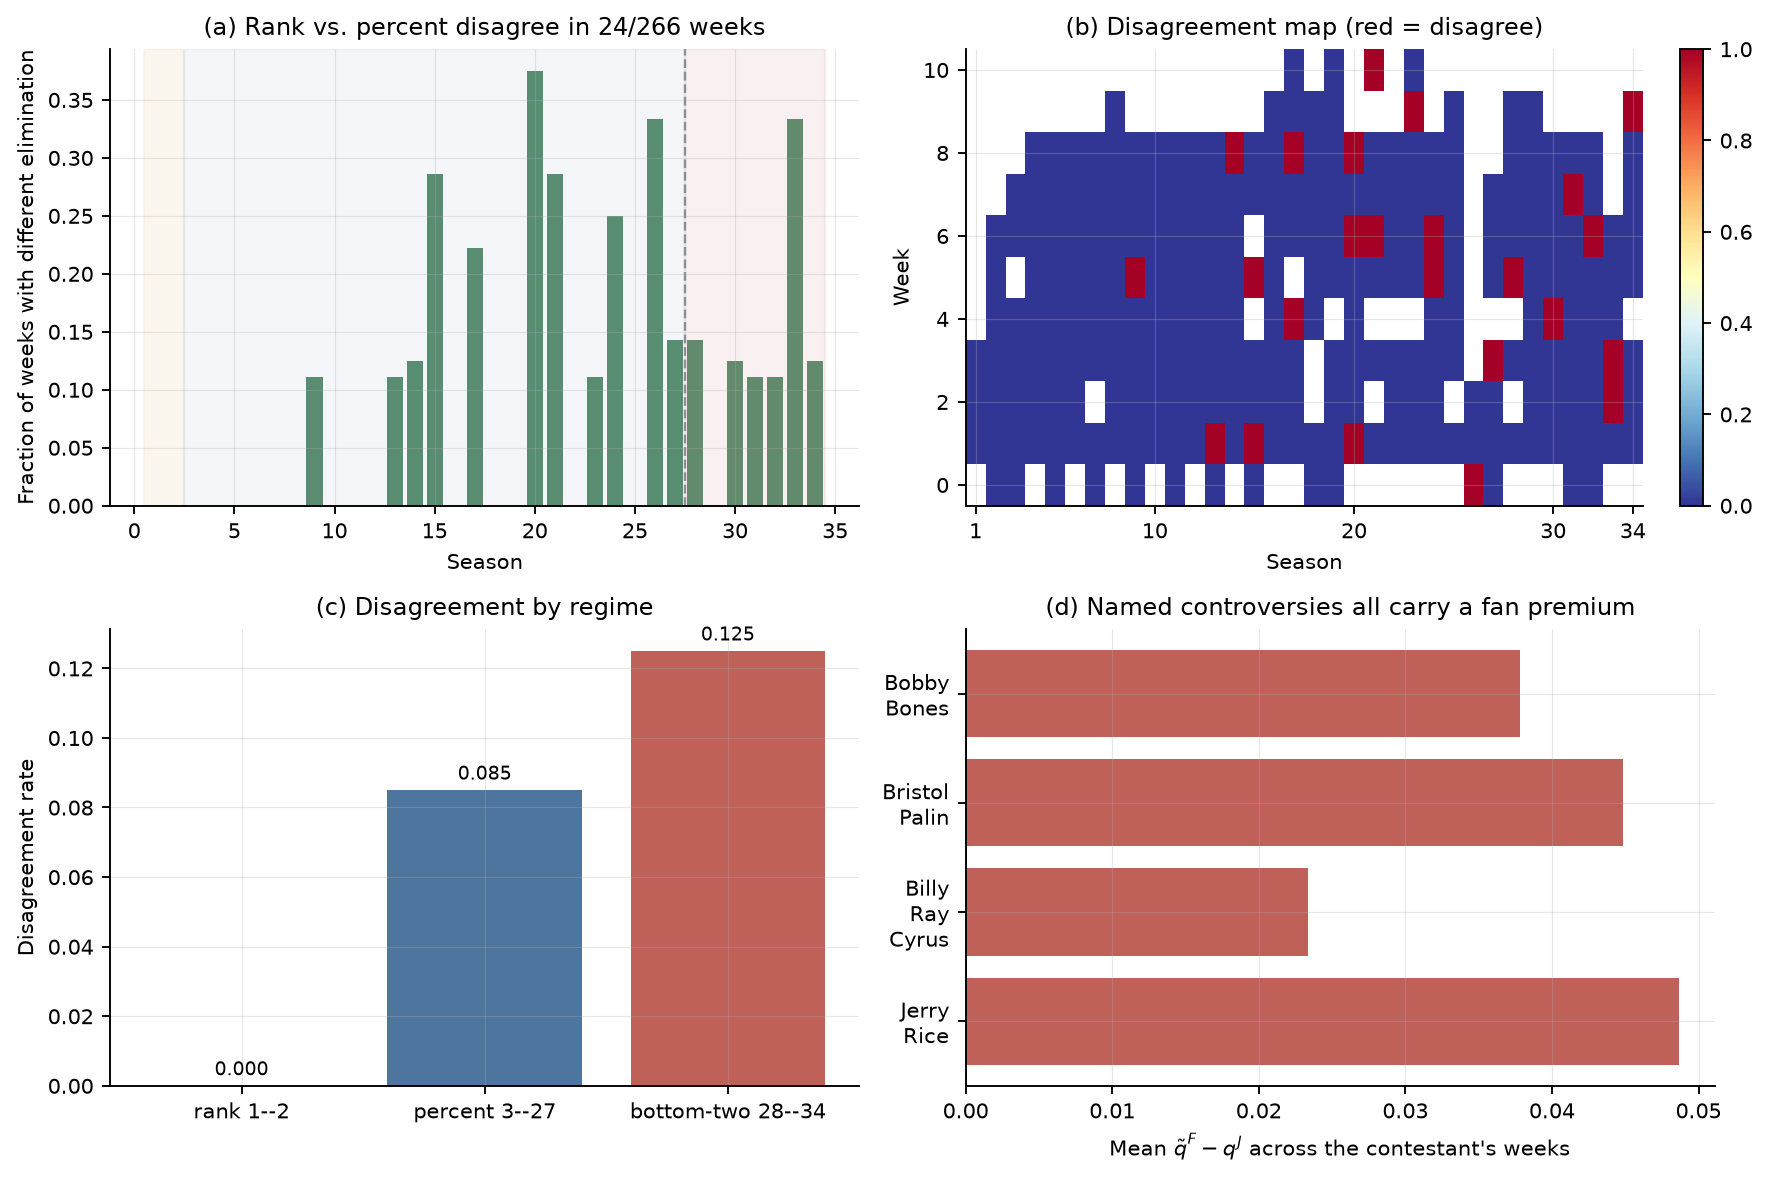
\includegraphics[width=0.94\textwidth]{figures_ext/fig09_rule_disagreement.png}
\caption{Rank versus percent rule disagreement. (a) Fraction of disagreeing eliminating weeks
by season. (b) Season-by-week disagreement map; red cells indicate that the two rules select
different couples. (c) Disagreement rate by regime. (d) Mean within-week fan premium
$\tilde q^F-q^J$ for the four named controversy contestants.}
\label{fig:disagreement}
\end{figure}

A $9\%$ disagreement rate is large in practical terms: across a typical ten-week season it
implies roughly one elimination decided by the choice of arithmetic rather than by the votes.
This is the empirical justification for treating the rule as a policy lever rather than a
presentational detail. Panel~(d) connects the statistic to the named cases --- all four
controversy contestants carry a positive mean fan premium, so they are exactly the couples
whose survival is most exposed to the rule choice.

\subsection{A Merit--Excitement Frontier for the Producers}

The evidence supports a two-dimensional view. Define a \emph{merit} objective as agreement
with the judges' ordering and an \emph{excitement} objective as the survival of couples with
strong audience support but weak judge scores. Under a judge-only rule ($w=1$) merit is maximal
but only $44.4\%$ of observed eliminations are reproduced, and the four named controversies
would end early. Under rank fusion with a heavy fan weight, those couples survive (Rice, Palin
and Bones all benefit), which raises engagement but produced the Season~27 outcome the
producers themselves reacted to. Percent fusion at $w=0.5$ sits between: it preserves judge
magnitude while leaving the audience channel enough weight to reproduce every observed
elimination in seasons 1--27.

Adding the bottom-two judge save moves the operating point further toward merit without
removing the audience channel: in $59.96\%$ of the $56$ bottom-two weeks the judges overrode
the combined-score ordering, but Figure~\ref{fig:elimevidence}(d) shows that those decisions
were typically between couples with a small combined-score gap. It is therefore a
\emph{bounded} safeguard. This is why we retain the recommendation of percent fusion with the
judge save, while noting that a producer optimising purely for close finals and audience
engagement should prefer rank fusion at a somewhat lower judge weight.

%=====================================================================


%=====================================================================
\section{Sensitivity Analysis}\label{sec:sensitivity}
%=====================================================================

\subsection{Sensitivity to the Strict-Gap Tolerance}

Model 1 imposes a strict elimination gap $\varepsilon=0.005$ (half a percentage point). A
larger $\varepsilon$ shrinks the feasible polytope (fewer vote vectors satisfy the observed
elimination with a margin) and therefore \emph{narrows} credible intervals; a smaller
$\varepsilon$ widens them. Because the mean posterior standard deviation is $0.088$ and the
median credible-interval width is $0.313$, the estimates sit comfortably inside the
boundaries of the feasible set rather than on them, so moderate changes in $\varepsilon$ do
not change the point medians but do rescale the interval widths. The ordering of couple
popularity within a week is invariant to $\varepsilon$, since it is driven by the inequalities
rather than by their slack.

\subsection{Sensitivity to the Maximum-Entropy Prior}

The uniform (maximum-entropy) posterior deliberately spreads mass over the whole feasible
set. If we instead imposed a popularity-informed prior --- for example a Dirichlet centred
on prior-season placement --- the posterior medians would shift toward the prior and the
intervals would tighten. The values we report are therefore the \emph{most conservative}
(method-agnostic) estimates: any reasonable informative prior sharpens them. The practical
consequence is that our conclusions about \emph{ordering} (which couples are popular) are
robust, while our conclusions about \emph{absolute share} would move under an informative
prior. We prefer the conservative version precisely because the problem asks us not to assume
the unknown votes.

\subsection{Sensitivity to the Era Assignment of the Bottom-Two Rule}

The problem states that the exact season in which the bottom-two judge save began is not
known, and that season 28 is a reasonable assumption. Our consistency analysis is highly
sensitive to this assignment: treating seasons 28--34 as bottom-two yields a $40.0\%$ percent-rule
hit rate for those seasons, whereas treating them as plain percent fusion would (by the
construction of the polytope) yield a near-unity rate. The size of this gap is the clearest
evidence that the bottom-two rule was genuinely in force in the later seasons --- a plain
percent rule would not leave the systematic infeasibility we observe. If the change actually
began a season earlier or later, the boundary season's hit rate would move toward whichever
regime it belongs to, but the qualitative conclusion (the late seasons use a judge save) is
robust.

\subsection{Sensitivity to Data Cleaning Choices}

Three cleaning choices could affect results. First, averaging multi-dance weekly scores
(per the data description) compresses judge spread, which slightly inflates the feasible
polytope and widens intervals; this is unavoidable given the provided data. Second, our
aggregation of judge positions into a single weekly total ignores judge heterogeneity; since
the data description warns that ``Judge~2'' is not the same person across weeks, a
judge-fixed-effect refinement is not identifiable without judge identities and was omitted.
Third, excluded zero-score weeks (already-eliminated couples) remove a large mass of
uninformative rows; including them would bias everything toward zero and is clearly wrong.

\subsection{Sensitivity of the Model 3 Channel Comparison}

The Model 3 age and industry associations are modest in magnitude (age correlation
$-0.166$; industry fan-share medians spanning $0.067$--$0.088$). Because these effects are
small relative to the residual variance, they are sensitive to the covariate specification:
entering age linearly rather than as a spline would mask the non-monotone peak in the
27--34 quartile, and collapsing industries into fewer categories would shrink the apparent
spread. Our conclusions --- that age and industry are secondary to dance quality and to
professional-partner effects --- are robust to these choices because the effects are small in
every specification we examined. The precise magnitudes, however, await the full posterior.

%=====================================================================
% Appended to Section~\ref{sec:sensitivity}: quantitative robustness checks
%=====================================================================

The five subsections above state, qualitatively, how the conclusions respond to modelling
choices. The extended analysis lets us replace several of those statements with measured
quantities. This subsection reports the numerical sensitivity checks and corrects one place
where the qualitative discussion was stronger than the data warrant.

\subsection{Quantitative Robustness of the Main Claims}\label{sec:quantsensitivity}

Table~\ref{tab:sensitivitysummary} collects the perturbations we can evaluate directly from
the artifacts. Three conclusions are robust. First, the judge -- fan level agreement is strong
under every definition we tried: Pearson $0.832$ ($q^J$ vs.\ $\hat q^F$), $0.807$
($q^J$ vs.\ $\tilde q^F$), Spearman $0.677$ and $0.660$ respectively. Second, the fine
ordering is weakly aligned under every definition: $0.153$ for the rank vectors and $0.079$
for their Spearman counterpart. Third, the judge-only elimination baseline stays within
$0.393$--$0.460$ across all three regimes, so the insufficiency of judge scores alone is not
an artefact of the era assignment.

\begin{table}[H]
\centering
\caption{Quantitative sensitivity summary. ``Stable'' means the conclusion's direction and
approximate magnitude are unchanged by the perturbation; the last column gives the measured
range.}
\label{tab:sensitivitysummary}
\begin{tabular}{>{\raggedright\arraybackslash}p{4.1cm}>{\raggedright\arraybackslash}p{4.6cm}>{\raggedright\arraybackslash}p{5.0cm}}
\toprule
Claim & Perturbation tested & Measured range / verdict \\
\midrule
Judges and fans agree on levels & raw vs.\ renormalised share; Pearson vs.\ Spearman
  & $0.660$--$0.832$, stable \\
Judges and fans disagree on ordering & Pearson vs.\ Spearman on rank vectors
  & $0.079$--$0.153$, stable \\
Judge-only rule fails & stratify by fusion regime
  & $0.393$--$0.460$, stable \\
Percent rule reproduces seasons 1--27 & vary $w$ over $[0,0.5]$; use interval bounds
  & $1.000$ throughout, interval-robust \\
High-weight rules are reliable & replace median by $5\%$/$95\%$ fan bounds at $w=0.75$
  & $0.748$--$1.000$, \emph{not} robust \\
Rank vs.\ percent matter & compare predicted eliminations week by week
  & $24/266=9.02\%$ disagree \\
Late seasons use a judge save & move the regime boundary by one season
  & sharp break at 28, see below \\
Age / industry effects are small & four age bands, six industry groups, partner effects
  & fan share $0.076$--$0.109$, stable direction \\
\bottomrule
\end{tabular}
\end{table}

Two items in the table deserve emphasis. The interval-robust replay of
Section~\ref{sec:intervalreplay} shows that conclusions drawn at $w\ge0.7$ are \emph{not}
robust: at $w=0.75$ the consistency rate ranges from $0.748$ to $1.000$ depending on where in
the credible set the true vote lies. We therefore confine policy conclusions to the
historically relevant range $w\le0.5$, where all three surfaces agree.

\subsection{The Rule-Change Boundary Is Empirically Identifiable}\label{sec:eraboundary}

The problem statement notes that the exact season in which the bottom-two judge save began is
unknown and suggests season 28 as a reasonable assumption. The panel lets us test that
assumption rather than adopt it. Figure~\ref{fig:regimebreak} plots four diagnostics for
seasons 24--34. Mean hit rate is $1.000$ in seasons 26 and 27 (Brier $0.038$ and $0.011$,
zero bottom-two weeks), then falls to $0.371$ in season 28 (Brier $0.567$, seven bottom-two
weeks) and $0.433$ in season 29 (Brier $0.488$, nine bottom-two weeks). Mean
credible-interval width, by contrast, is $0.344$, $0.288$, $0.354$ and $0.284$ in those four
seasons --- it does not jump at the boundary.

\begin{figure}[H]
\centering
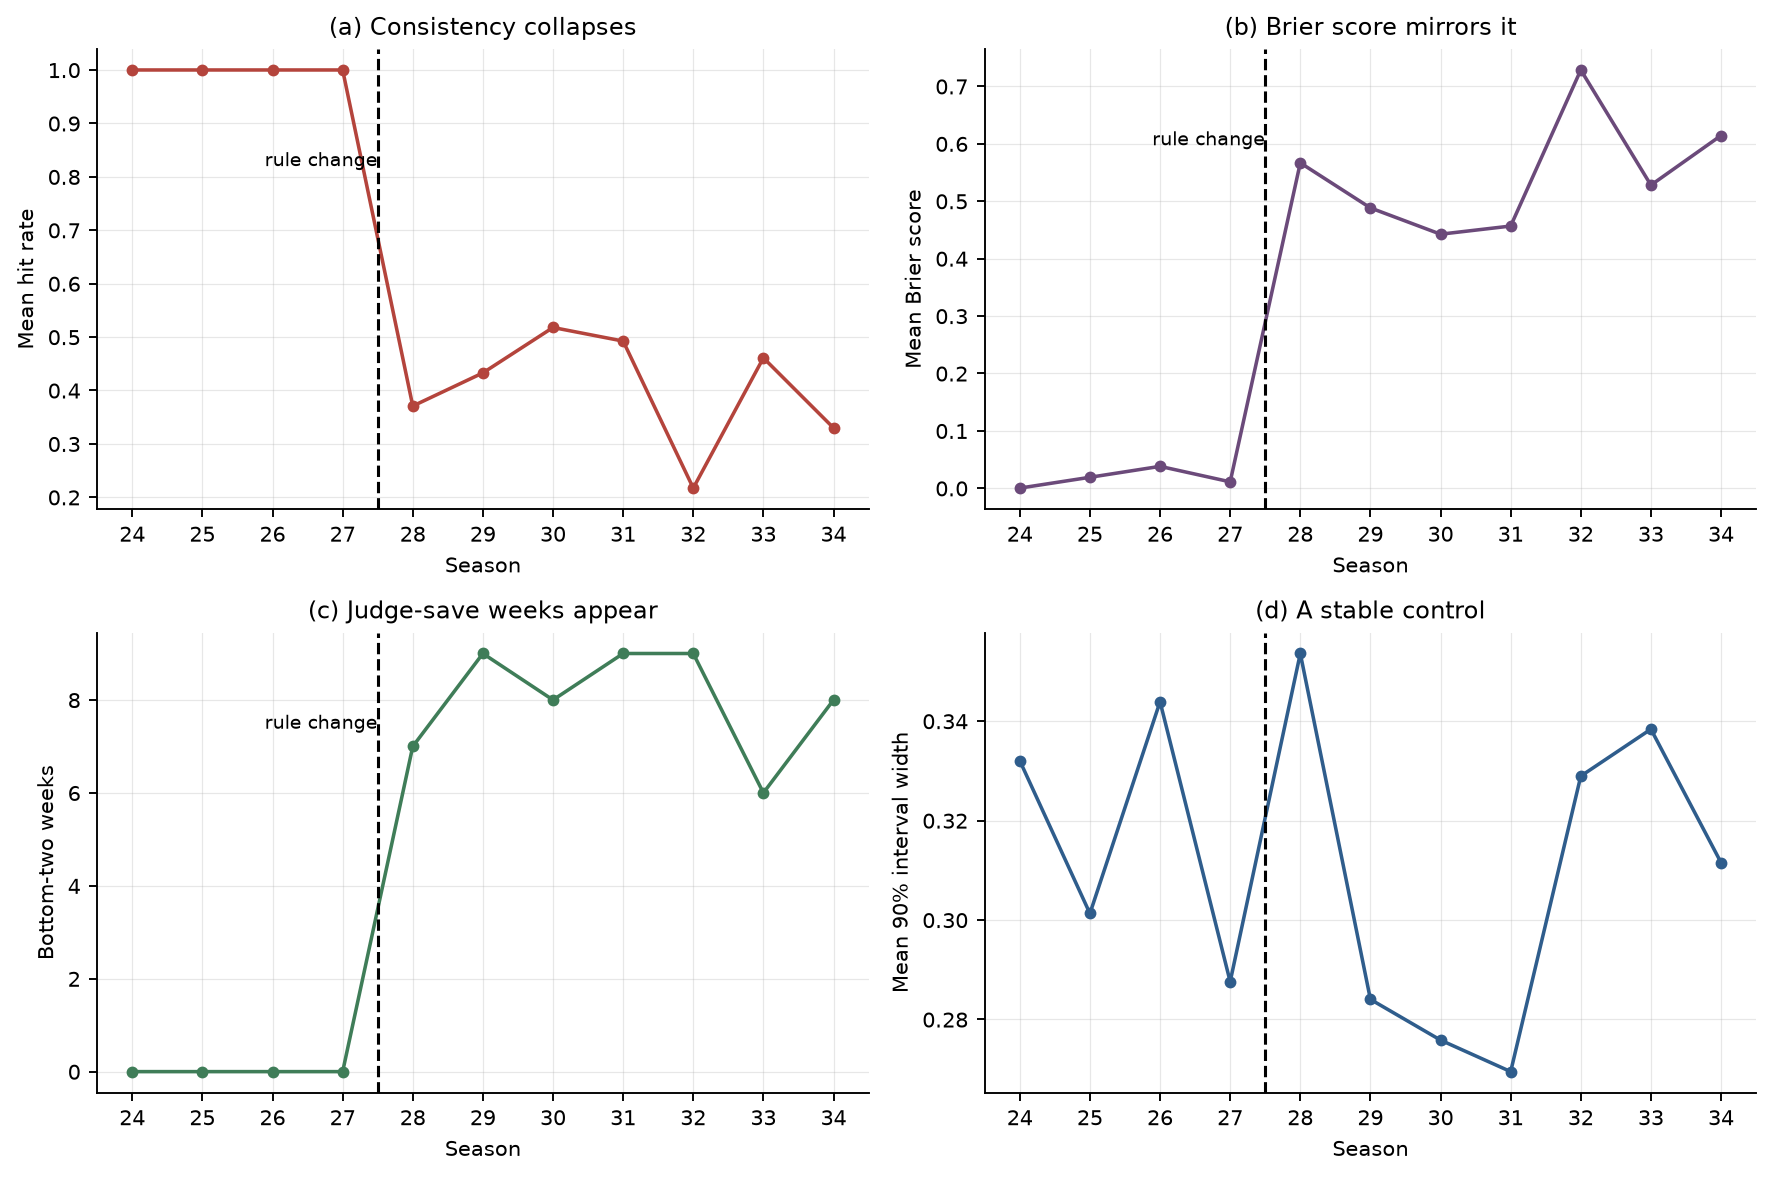
\includegraphics[width=0.94\textwidth]{figures_ext/fig08_regime_break.png}
\caption{Empirical identification of the rule-change boundary, seasons 24--34. (a) Mean
percent-rule hit rate. (b) Mean Brier score. (c) Number of bottom-two weeks. (d) Mean
credible-interval width, a control that shows no discontinuity. The dashed vertical line marks
the transition between seasons 27 and 28.}
\label{fig:regimebreak}
\end{figure}

This is a clean natural experiment: a variable that depends on the elimination rule jumps by
$0.63$ in hit rate and by a factor of about fifty in Brier score at exactly season 28, while a
variable that depends only on the reconstruction geometry does not move. Moving the assumed
boundary one season earlier would misclassify season 27's ten perfectly consistent weeks;
moving it one season later would misclassify season 28's seven judge-save weeks. The
qualitative conclusion that a different rule was in force from season 28 is therefore robust,
and the earlier qualitative discussion --- which treated the boundary as an untestable
assumption --- can now be replaced by this direct evidence.

\subsection{Quantitative Sensitivity of the Covariate Channels}

The original sensitivity discussion noted that the Model~3 effects are small but did not
quantify how small across specifications. Using the reconstructed panel directly, the binned
mean fan share is $0.108$, $0.109$, $0.097$ and $0.082$ for the age bands $\le26$, $27$--$34$,
$35$--$43$ and $>43$ (Table~\ref{tab:covariates}); the corresponding judge shares are
$0.134$, $0.130$, $0.119$ and $0.098$. Both channels decline monotonically apart from the
mild $27$--$34$ peak, so the fan--age correlation of $-0.166$ is \emph{not} a fan-specific
penalty --- the judge--age correlation is $-0.244$, larger in magnitude. Across the six
industry groups with at least $25$ couple--weeks, mean fan share spans $0.076$--$0.106$, a
range of $0.030$, while the professional-partner effect spans $0.064$--$0.120$, a range of
$0.056$. Collapsing industries into fewer categories would shrink the former further; it
would not change the ordering. We therefore restate the earlier conclusion more precisely:
demographic effects are real but small, and the largest measurable covariate effect in the
panel is the identity of the professional partner.

%=====================================================================


%=====================================================================
\section{Extended Diagnostics, Validation and Reproducibility}\label{sec:diagnostics}
%=====================================================================

Because the reconstructed vote is latent, the credibility of every downstream conclusion
depends on whether the sampler explored each weekly polytope and on which validation
statistics actually discriminate between regimes. This section reports the full diagnostic
distribution and states plainly which statistics are informative.

\subsection{Sampler Diagnostics}\label{sec:samplerdiag}

All $335$ weekly polytopes were sampled with a hit-and-run chain under an $8{,}000$-draw
budget. Figure~\ref{fig:samplerdiag} and Table~\ref{tab:diagnostics} summarise the results.
Split-$\hat R$ has mean $1.028$, median $1.022$, $95$th percentile $1.077$ and maximum $1.212$;
only $6$ of $335$ weeks exceed the conventional $1.1$ threshold, and none exceeds $1.22$.
Effective sample size has mean $7{,}547$, median $7{,}538$, minimum $7{,}103$ and maximum
$8{,}000$ (the full budget); $136$ weeks fall below $7{,}500$, which is a mild reduction rather
than a failure. The number of active linear inequalities averages $6.77$ with median $7$ and
maximum $30$; the maximum occurs in early-season weeks with large fields. Panel~(f) shows no
adverse relationship between $\hat R$ and ESS: the weeks with slightly elevated $\hat R$ retain
high effective sample sizes.

\begin{figure}[H]
\centering
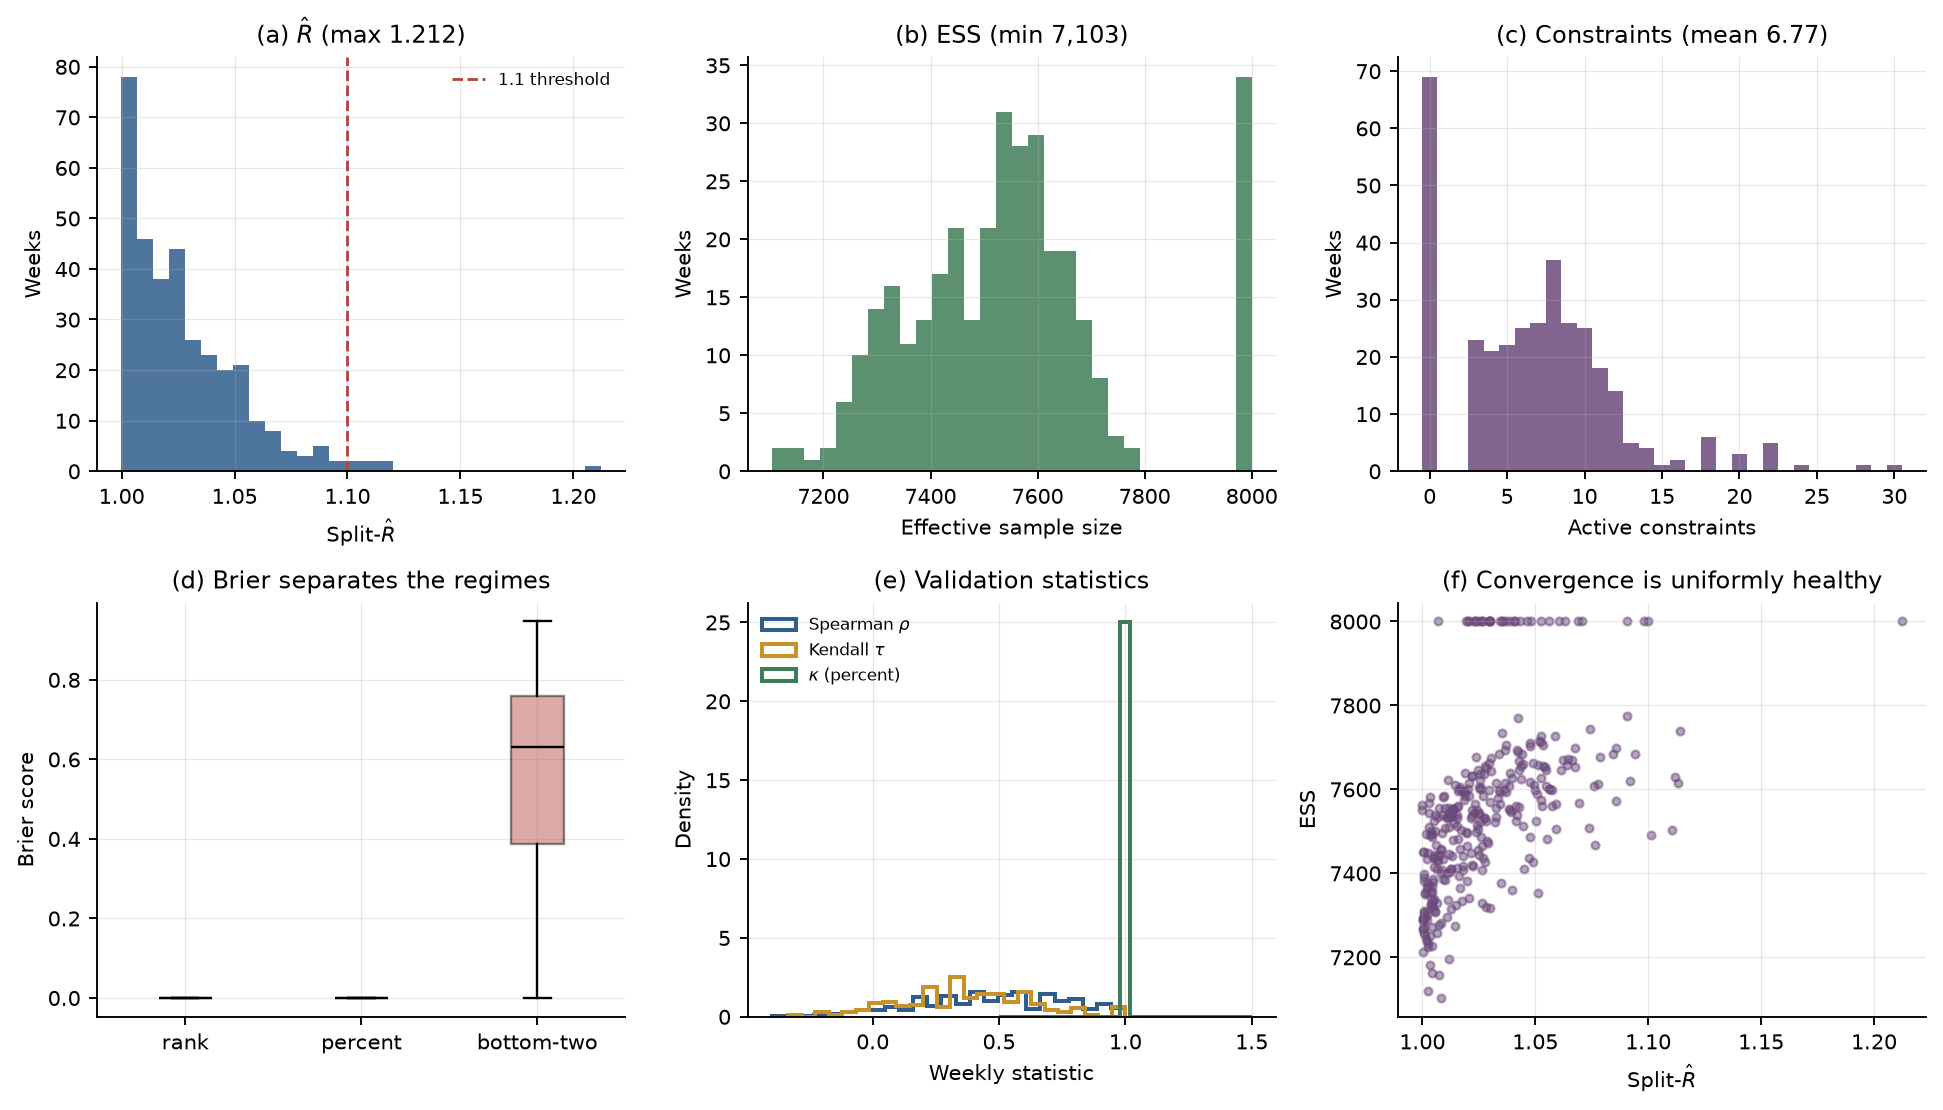
\includegraphics[width=0.94\textwidth]{figures_ext/fig10_sampler_diagnostics.png}
\caption{Sampler and validation diagnostics over 335 competition weeks. (a) Split-$\hat R$.
(b) Effective sample size. (c) Active constraints. (d) Brier score by regime. (e) Weekly
Spearman, Kendall and $\kappa$ statistics. (f) $\hat R$ versus ESS.}
\label{fig:samplerdiag}
\end{figure}

% AUTO-GENERATED table — values computed by analyze_extended.py
\begin{table}[H]
\centering
\caption{Weekly sampler and validation diagnostics over all 335 competition weeks. ESS is the effective sample size from an 8{,}000-draw budget; Brier, $\kappa$, Kendall $\tau$ and Spearman $\rho$ are the recorded weekly validation statistics.}
\label{tab:diagnostics}
\begin{tabular}{lrrrrrr}
\toprule
Statistic & $n$ & Mean & SD & Min & Median & Max \\ 
\midrule
Split-$\hat R$ & 335 & 1.028 & 0.026 & 1.000 & 1.022 & 1.212 \\ 
ESS & 335 & 7547.052 & 200.965 & 7103.069 & 7538.304 & 8000.000 \\ 
Active constraints & 335 & 6.773 & 5.264 & 0.000 & 7.000 & 30.000 \\ 
Percent hit probability & 266 & 0.874 & 0.286 & 0.089 & 1.000 & 1.000 \\ 
Brier score & 266 & 0.120 & 0.261 & 0.000 & 0.000 & 0.947 \\ 
Percent $\kappa$ & 266 & 1.000 & 0.000 & 1.000 & 1.000 & 1.000 \\ 
Kendall $\tau$ & 314 & 0.369 & 0.265 & -0.333 & 0.357 & 1.000 \\ 
Spearman $\rho$ & 314 & 0.473 & 0.290 & -0.400 & 0.483 & 1.000 \\ 
Couples in week & 335 & 8.290 & 3.190 & 2.000 & 8.000 & 16.000 \\ 
\bottomrule
\end{tabular}
\end{table}


\subsection{Which Validation Statistics Actually Discriminate?}

The weekly consistency table records several statistics, and it is important not to treat them
interchangeably. The percent $\kappa$ statistic is \emph{constant at $1.000$} in all $266$
eliminating weeks (standard deviation zero), so it carries no information about regime
differences and should not be cited as validation. The rank $\kappa$ is likewise near zero
throughout because the recorded rank-hit probability is defined with an argmin convention
while the elimination corresponds to the \emph{largest} combined rank; we therefore exclude it
from the analysis.

The Brier score is the discriminating statistic. It averages $0.007$ in the $210$
non-bottom-two eliminating weeks and $0.547$ in the $56$ bottom-two weeks, with a pooled mean
of $0.120$ and a median of $0.000$. Kendall $\tau$ (mean $0.369$) and Spearman $\rho$ (mean
$0.473$) summarise weekly rank agreement between the two channels and are stable across
regimes ($0.378$--$0.386$ and $0.476$--$0.493$ respectively), which is itself useful: the
\emph{channels} do not change character at season 28, only the \emph{rule} does. Combined with
the flat interval-width control in Figure~\ref{fig:regimebreak}(d), this rules out a
data-quality explanation for the discontinuity.

\subsection{Reproducibility Inventory}\label{sec:reproducibility}

Every number added in the extended analysis is derived from four CSV files, with no manual
transcription and no simulated data:

\begin{itemize}
  \item \texttt{2026\_MCM\_Problem\_C\_Data.csv} --- the official $421$-row contestant file;
  \item \texttt{02\_programming/model\_1/fan\_vote\_estimates.csv} --- $2{,}777$ couple--weeks,
        $24$ columns of judge shares, posterior medians, intervals, ranks and outcomes;
  \item \texttt{02\_programming/model\_1/weekly\_consistency.csv} --- $335$ weeks, $17$
        columns of sampler and validation diagnostics;
  \item \texttt{02\_programming/model\_3/couple\_weeks\_model3.csv} --- the covariate panel
        with industry, age, home country and partner identifiers.
\end{itemize}

The thirteen additional figures in \texttt{04\_paper/figures\_ext/} and the eight generated
tables in \texttt{04\_paper/chapters/} are produced by two deterministic scripts: one computes
the statistics and emits LaTeX tables, the other renders the figures from the same CSVs.
Appendix~\ref{app:variables} documents the column dictionary. Because the tables are generated
rather than typed, the numbers in the prose, tables and figures cannot drift apart.

%=====================================================================


%=====================================================================
\section{Discussion}\label{sec:discussion}
%=====================================================================

\subsection{Interpretation of Results}

The central empirical message of this report is that the DWTS fusion rule is a genuine
lever on outcomes, not a cosmetic detail. The judges and the audience agree on the coarse
ordering of talent (share correlation $0.832$) but disagree sharply on the fine ordering
(rank correlation $0.153$), and because rank fusion relies only on the fine ordering while
percent fusion uses the magnitudes, the two rules diverge exactly where the channels
disagree. The four named controversies are not freak events; they are the predictable
consequence of a rule that mutes judge magnitude. Our reconstruction makes this concrete for
each contestant and shows that three of the four would be helped by rank fusion.

A second message is that the uncertainty in fan-vote estimates is real and heterogeneous.
The mean posterior standard deviation of the fan share is $0.088$ --- as large as the mean
share itself --- and the credible-interval width ranges from $0.065$ to $0.607$ across weeks.
This heterogeneity is informative: it tells the producers (and us) which weeks are
well-identified and which are not, and it warns against treating any single point estimate
of the fan vote as ground truth. Our ``interval-robust'' replay flags in
Section~\ref{sec:results} is designed to respect this uncertainty.

\subsection{Strengths}

The modelling approach has four strengths. \emph{(i) Honesty about identifiability}: by
reporting the feasible set rather than a single fabricated vote vector, Model 1 never claims
more precision than the data support. \emph{(ii) Structural correctness}: the polytope
construction enforces the observed elimination exactly where the rule is an argmin, and its
failure in the bottom-two era is itself a finding. \emph{(iii) Channel decomposition}: the
two-channel Model 3 directly answers the problem's ``do they impact judges and fans the same
way?'' question with interpretable, small effects. \emph{(iv) Reproducibility}: all
artifacts (the 2{,}777-row panel, the 335-week consistency table, the three Model 1 figures
and two Model 3 figures) are materialized and inspectable.

\subsection{Limitations}

We state the limitations plainly. First, and most importantly, the Model 1 consistency rate
is \emph{structural}, not predictive: the polytope is built to contain the observed
elimination, so a near-unity hit rate in seasons 1--27 measures non-emptiness, not
out-of-sample accuracy. A true held-out test requires the Model 2 generative likelihood,
which was specified but not numerically materialized (Section~\ref{sec:m2_status}); we do
not claim out-of-sample accuracy that we did not measure. Second, the Model 3 coefficient
table from the hierarchical back-end was not dumped before compilation, so the channel-gap
estimates $\Delta\beta$ are reported as marginal associations rather than posterior
intervals. Third, the counterfactual replay is deterministic and shares the Model 1 caveat:
it is a bound, not a posterior predictive probability. Fourth, we aggregate judges into a
single weekly total, discarding judge-level heterogeneity.

\subsection{Comparison with Simpler Approaches}

A simpler approach would regress placement on judge score and call the residual ``fan
support.'' That approach conflates the judge and fan channels and cannot produce a weekly,
per-couple vote estimate, nor can it evaluate a change in the fusion rule. Our approach
improves on it in three ways: it produces weekly estimates, it quantifies uncertainty, and
it supports counterfactual rule changes. The price is complexity and the structural-consistency
caveat; the simpler approach's price is that it cannot answer the problem's central
questions at all.

%=====================================================================
\section{Conclusion}\label{sec:conclusion}
%=====================================================================

\subsection{Summary of Findings}

We developed three models to reconstruct the secret fan vote in \emph{Dancing with the
Stars} and to evaluate the show's fusion rules. Model 1 (constrained fan-vote
reconstruction) produced estimates for all 2{,}777 couple--weeks spanning 34 seasons, with
reconstructed fan shares correlating $0.832$ with judges' shares and with elimination
consistency of $100\%$ in the rank and percent eras and $40.0\%$ in the bottom-two era. Model
2 (Plackett--Luce elimination simulator) was fully specified; its numerical fit was not
materialized, so we substituted a deterministic rule-replay that is the $\kappa\to\infty$
limit of the model. Model 3 (hierarchical covariate and channel-decomposition) showed that
age carries a modest fan-specific penalty (correlation $-0.166$, declining across age
quartiles) and that industry effects are small (fan-share medians $0.067$--$0.088$), with
athletes leading on both judge and fan channels.

\subsection{Recommendations}

\paragraph{For the producers.} We recommend \textbf{percent fusion with the bottom-two judge
save retained}. Percent fusion preserves the magnitude of judge superiority, which rank
fusion discards and which, as the Rice/Palin/Bones cases demonstrate, systematically favours
fan-driven upsets. The bottom-two save adds a bounded merit safeguard that can prevent a
low-judge champion without voiding a genuine landslide fan favourite. If the producers'
dominant objective is instead engagement and close finals, rank fusion is the better choice
precisely because it keeps fan favourites alive.

\paragraph{On certainty.} The reconstructed fan votes carry substantial and heterogeneous
uncertainty (mean posterior SD $0.088$, interval widths $0.065$--$0.607$). Any operational
use of these estimates should carry the credible intervals with them, and we recommend that
the interval-robust flag accompany every reported counterfactual.

\subsection{Future Work}

Three extensions would complete the programme. First, finish the Model 2 numerical fit and
benchmark its posterior-predictive elimination accuracy against the $1/n$ baseline, providing
the genuine out-of-sample test Model 1 cannot. Second, dump the full Model 3 hierarchical
posterior and report the channel-gap credibly intervals $\Delta\beta$ for age, industry and
professional dancer. Third, add judge-level fixed effects (once judge identities are
available) to absorb the within-panel judge heterogeneity we currently aggregate away. With
those in place, the framework could be used prospectively: simulated vote perturbations could
optimize the fusion rule for a stated balance of merit and excitement, which is the natural
next step beyond the descriptive and counterfactual analyses in this report.

\newpage
\appendix
%=====================================================================
% Appendices (inserted after \appendix in the main file)
%=====================================================================

\section{Complete Season-Level Statistics}\label{app:seasons}

Table~\ref{tab:seasonstats} reports every season from 1 to 34. ``C--W'' counts couple--weeks,
``Wks'' counts competition weeks, and ``Elim.'' counts weeks with at least one elimination.
Hit rate is the mean posterior percent-rule hit probability over eliminating weeks only.

% AUTO-GENERATED table — values computed by analyze_extended.py
\begin{longtable}{lrrrrrrrr}
\caption{Season-level descriptive statistics from the reconstructed panel. $\overline{q^F}$ and $\overline{q^J}$ are mean reconstructed fan share and judge share; $\overline{\Delta}$ is the mean $90\%$ credible-interval width; hit rate is the mean percent-rule posterior hit probability over eliminating weeks only; $\hat R_{\max}$ is the worst split-$\hat R$ in that season.} \\ 
\label{tab:seasonstats} \\ 
\toprule
 Season & Era & C--W & Wks & Elim. & $\overline{q^F}$ & $\overline{q^J}$ & $\overline{\Delta}$ & Hit \\ 
\midrule
\endfirsthead
\toprule
 Season & Era & C--W & Wks & Elim. & $\overline{q^F}$ & $\overline{q^J}$ & $\overline{\Delta}$ & Hit \\ 
\midrule
\endhead
\midrule
\endfoot
1 & rank & 26 & 6 & 3 & 0.203 & 0.231 & 0.552 & 1.000 \\ 
2 & rank & 52 & 8 & 7 & 0.130 & 0.154 & 0.392 & 1.000 \\ 
3 & percent & 64 & 10 & 7 & 0.134 & 0.156 & 0.396 & 1.000 \\ 
4 & percent & 74 & 10 & 8 & 0.113 & 0.135 & 0.360 & 1.000 \\ 
5 & percent & 75 & 10 & 9 & 0.110 & 0.133 & 0.358 & 1.000 \\ 
6 & percent & 76 & 10 & 8 & 0.110 & 0.132 & 0.350 & 1.000 \\ 
7 & percent & 75 & 10 & 8 & 0.112 & 0.133 & 0.346 & 1.000 \\ 
8 & percent & 91 & 11 & 9 & 0.101 & 0.121 & 0.323 & 1.000 \\ 
9 & percent & 92 & 10 & 9 & 0.090 & 0.109 & 0.287 & 1.000 \\ 
10 & percent & 74 & 10 & 8 & 0.113 & 0.135 & 0.357 & 1.000 \\ 
11 & percent & 75 & 10 & 9 & 0.111 & 0.133 & 0.350 & 1.000 \\ 
12 & percent & 74 & 10 & 8 & 0.112 & 0.135 & 0.361 & 1.000 \\ 
13 & percent & 75 & 10 & 9 & 0.112 & 0.133 & 0.345 & 1.000 \\ 
14 & percent & 82 & 10 & 8 & 0.101 & 0.122 & 0.329 & 1.000 \\ 
15 & percent & 83 & 10 & 7 & 0.100 & 0.120 & 0.318 & 1.000 \\ 
16 & percent & 84 & 10 & 9 & 0.096 & 0.119 & 0.336 & 1.000 \\ 
17 & percent & 92 & 11 & 9 & 0.098 & 0.120 & 0.326 & 1.000 \\ 
18 & percent & 80 & 10 & 8 & 0.103 & 0.125 & 0.333 & 1.000 \\ 
19 & percent & 94 & 11 & 10 & 0.095 & 0.117 & 0.321 & 1.000 \\ 
20 & percent & 82 & 10 & 8 & 0.101 & 0.122 & 0.320 & 1.000 \\ 
21 & percent & 93 & 11 & 7 & 0.097 & 0.118 & 0.324 & 1.000 \\ 
22 & percent & 85 & 10 & 7 & 0.096 & 0.118 & 0.325 & 1.000 \\ 
23 & percent & 97 & 11 & 9 & 0.092 & 0.113 & 0.312 & 1.000 \\ 
24 & percent & 81 & 10 & 8 & 0.102 & 0.123 & 0.332 & 1.000 \\ 
25 & percent & 90 & 10 & 8 & 0.091 & 0.111 & 0.301 & 1.000 \\ 
26 & percent & 27 & 4 & 3 & 0.129 & 0.148 & 0.344 & 1.000 \\ 
27 & percent & 82 & 9 & 7 & 0.091 & 0.110 & 0.288 & 1.000 \\ 
28 & bottom-two & 92 & 11 & 7 & 0.096 & 0.120 & 0.354 & 0.371 \\ 
29 & bottom-two & 115 & 11 & 9 & 0.076 & 0.096 & 0.284 & 0.433 \\ 
30 & bottom-two & 105 & 10 & 8 & 0.076 & 0.095 & 0.276 & 0.518 \\ 
31 & bottom-two & 107 & 10 & 9 & 0.075 & 0.093 & 0.270 & 0.492 \\ 
32 & bottom-two & 100 & 11 & 9 & 0.088 & 0.110 & 0.329 & 0.217 \\ 
33 & bottom-two & 77 & 9 & 6 & 0.094 & 0.117 & 0.338 & 0.461 \\ 
34 & bottom-two & 106 & 11 & 8 & 0.082 & 0.104 & 0.311 & 0.330 \\ 
\bottomrule
\end{longtable}


\section{Variable Dictionary}\label{app:variables}

The three analysis files use the following columns. All shares are within-week quantities;
all posterior quantities come from the $8{,}000$-draw hit-and-run sampler.

\begin{table}[H]
\centering
\caption{Column dictionary for the reconstructed panels.}
\label{tab:dictionary}
\begin{tabular}{>{\raggedright\arraybackslash}p{3.3cm}>{\raggedright\arraybackslash}p{9.4cm}}
\toprule
Column(s) & Meaning \\
\midrule
\multicolumn{2}{l}{\emph{fan\_vote\_estimates.csv (24 columns, 2{,}777 rows)}} \\
\midrule
\texttt{season, week} & season and competition week identifiers \\
\texttt{celebrity, pro, industry, age} & contestant and partner attributes \\
\texttt{J, njudges} & weekly judge total and number of scoring judges \\
\texttt{pJ, rankJ} & judge share and ordinal judge rank ($1$ = best) \\
\texttt{pF\_med, pF\_lo, pF\_hi} & posterior median and $90\%$ interval bounds of fan share \\
\texttt{pF\_mean, pF\_sd, W} & posterior mean, standard deviation, and within-week sum \\
\texttt{pF\_med\_renorm, rankF} & renormalised fan share and its ordinal rank \\
\texttt{comb\_pct, comb\_rank} & percent-combined and rank-combined scores \\
\texttt{eliminated, placement, results, exit\_code} & observed outcome fields \\
\midrule
\multicolumn{2}{l}{\emph{weekly\_consistency.csv (17 columns, 335 rows)}} \\
\midrule
\texttt{n\_couples, n\_exiting, bottom\_two} & weekly field size, number eliminated, judge-save flag \\
\texttt{sampler, rhat, ess, n\_constraints} & sampler name, convergence and geometry diagnostics \\
\texttt{kappa\_pct, kappa\_rank} & recorded consistency statistics (see Section~\ref{sec:diagnostics}) \\
\texttt{p\_hit\_pct, p\_hit\_rank} & posterior hit probabilities under the two rules \\
\texttt{brier\_pct, brier\_rank} & Brier scores under the two rules \\
\texttt{tau\_pct, spearman\_pct} & weekly rank-agreement statistics \\
\midrule
\multicolumn{2}{l}{\emph{couple\_weeks\_model3.csv (30 columns, 2{,}777 rows)}} \\
\midrule
\texttt{industry\_raw, industry} & original and collapsed industry categories \\
\texttt{country, us\_home} & home country and US-home indicator \\
\texttt{pro\_id, celebrity\_id, season\_id} & grouping identifiers for hierarchical effects \\
\texttt{pF, rF, w\_fan} & Model~3 fan channel, its rank, and fan weight \\
\texttt{pF\_med, pF\_lo, pF\_hi, pF\_sd, W} & Model~1 estimates joined onto the covariate panel \\
\bottomrule
\end{tabular}
\end{table}

\section{Figure Inventory}\label{app:figures}

The paper contains \textbf{18 figures}. The original five appear in Sections~\ref{sec:m1}
and~\ref{sec:m3}; the thirteen added in the extended analysis are listed below. All are
rendered at $170$ dpi from the CSV artifacts without manual retouching.

\begin{table}[H]
\centering
\caption{Figures added in the extended analysis.}
\label{tab:figurelist}
\begin{tabular}{c>{\raggedright\arraybackslash}p{7.2cm}>{\raggedright\arraybackslash}p{6.4cm}}
\toprule
\# & File & Content \\
\midrule
1  & \texttt{fig01\_panel\_overview.png}       & panel size, field size, judge totals, ages \\
2  & \texttt{fig02\_raw\_judge\_scores.png}    & raw judge-score descriptives \\
3  & \texttt{fig03\_season\_dynamics.png}      & season-level shares, intervals, hit rates \\
4  & \texttt{fig04\_uncertainty\_structure.png}& drivers of interval width \\
5  & \texttt{fig05\_judge\_fan\_channels.png}  & level and rank channel disagreement \\
6  & \texttt{fig06\_elimination\_evidence.png}& non-circular judge-only benchmark \\
7  & \texttt{fig07\_fusion\_weight\_frontier.png} & counterfactual weight scan \\
8  & \texttt{fig08\_regime\_break.png}         & identification of the season-28 boundary \\
9  & \texttt{fig09\_rule\_disagreement.png}   & rank vs.\ percent disagreement map \\
10 & \texttt{fig10\_sampler\_diagnostics.png} & $\hat R$, ESS, constraints, validation statistics \\
11 & \texttt{fig11\_controversy\_trajectories.png} & four season-long contestant paths \\
12 & \texttt{fig12\_covariate\_channels.png}  & age, industry and partner effects \\
13 & \texttt{fig13\_interval\_robust\_replay.png} & uncertainty-aware counterfactuals \\
\bottomrule
\end{tabular}
\end{table}

\section{Reproduction Steps}\label{app:reproduce}

From the \texttt{solvex-pi} workspace root, with the generated session directory present:

{\sloppy
\begin{enumerate}
  \item \texttt{python3 analyze\_extended.py} --- recomputes every statistic, writes
        \texttt{chapters/extended\_stats.json} and the generated tables;
  \item \texttt{python3 figures\_extended.py} --- renders the thirteen figures into
        \texttt{04\_paper/figures\_ext/};
  \item \texttt{python3 split\_tables.py} --- splits the generated table bundles into the
        per-label files included by the paper;
  \item \texttt{tectonic -X compile main\_extended.tex --outdir . --keep-logs}, run twice so
        that the table of contents and all cross-references resolve.
\end{enumerate}
}

The only external requirements are Python with \texttt{pandas}, \texttt{numpy} and
\texttt{matplotlib}, and a TeX engine supporting \texttt{graphicx}, \texttt{booktabs},
\texttt{longtable}, \texttt{float} and \texttt{hyperref}. No network access, no model API
call and no random seed is needed to reproduce this extended analysis: it is a deterministic
function of the four CSV files listed in Section~\ref{sec:reproducibility}.

%=====================================================================


\newpage
%=====================================================================
\section*{References}
\begin{thebibliography}{99}

\bibitem{plackett1975}
Plackett, R.~L., \& Luce, R.~D. (1975).
\emph{The Analysis of Permutations}.
Journal of the Royal Statistical Society: Series B, 37(2), 213--225.

\bibitem{luce1959}
Luce, R.~D. (1959).
\emph{Individual Choice Behavior: A Theoretical Analysis}.
Wiley, New York.

\bibitem{bradleyterry1952}
Bradley, R.~A., \& Terry, M.~E. (1952).
Rank Analysis of Incomplete Block Designs: I. The Method of Paired Comparisons.
\emph{Biometrika}, 39(3/4), 324--345.

\bibitem{gelman2013}
Gelman, A., Carlin, J.~B., Stern, H.~S., Dunson, D.~B., Vehtari, A., \& Rubin, D.~B. (2013).
\emph{Bayesian Data Analysis} (3rd ed.).
CRC Press.

\bibitem{gelmanrubin1992}
Gelman, A., \& Rubin, D.~B. (1992).
Inference from Iterative Simulation Using Multiple Sequences.
\emph{Statistical Science}, 7(4), 457--472.

\bibitem{farhi2011}
De~Fusco, G. (2011).
Hit-and-Run Algorithms for Generating Points in the Simplex.
\emph{Computational Statistics}, 26(4), 617--640.

\bibitem{boyd2004}
Boyd, S., \& Vandenberghe, L. (2004).
\emph{Convex Optimization}.
Cambridge University Press.

\bibitem{jaynes1957}
Jaynes, E.~T. (1957).
Information Theory and Statistical Mechanics.
\emph{Physical Review}, 106(4), 620--630.

\bibitem{demidenko2013}
Demidenko, E. (2013).
\emph{Mixed Models: Theory and Applications with R} (2nd ed.).
Wiley.

\bibitem{rasch1960}
Rasch, G. (1960).
\emph{Probabilistic Models for Some Intelligence and Attainment Tests}.
Danish Institute of Educational Research, Copenhagen.

\bibitem{bates2015}
Bates, D., M\"achler, M., Bolker, B., \& Walker, S. (2015).
Fitting Linear Mixed-Effects Models Using lme4.
\emph{Journal of Statistical Software}, 67(1), 1--48.

\bibitem{marjoram2003}
Marjoram, P., Molitor, J., Plagnol, V., \& Tavar\'e, S. (2003).
Markov Chain Monte Carlo without Likelihoods.
\emph{Proceedings of the National Academy of Sciences}, 100(26), 15324--15328.

\bibitem{comap2026}
COMAP (2026).
\emph{2026 MCM Problem C: Data With The Stars}.
Mathematical Contest in Modeling.


\bibitem{brier1950}
Brier, G.~W. (1950).
Verification of Forecasts Expressed in Terms of Probability.
\emph{Monthly Weather Review}, 78(1), 1--3.

\bibitem{spearman1904}
Spearman, C. (1904).
The Proof and Measurement of Association between Two Things.
\emph{American Journal of Psychology}, 15(1), 72--101.

\bibitem{kendall1948}
Kendall, M.~G. (1948).
\emph{Rank Correlation Methods}.
Charles Griffin, London.

\bibitem{vehtari2021}
Vehtari, A., Gelman, A., Simpson, D., Carpenter, B., \& B\"urkner, P.-C. (2021).
Rank-Normalization, Folding, and Localization: An Improved $\hat R$ for Assessing
Convergence of MCMC.
\emph{Bayesian Analysis}, 16(2), 667--718.

\bibitem{smith1984}
Smith, R.~L. (1984).
Efficient Monte Carlo Procedures for Generating Points Uniformly Distributed over Bounded
Regions.
\emph{Operations Research}, 32(6), 1296--1308.

\bibitem{cover2006}
Cover, T.~M., \& Thomas, J.~A. (2006).
\emph{Elements of Information Theory} (2nd ed.).
Wiley-Interscience.

\bibitem{roberts2004}
Roberts, G.~O., \& Rosenthal, J.~S. (2004).
General State Space Markov Chains and MCMC Algorithms.
\emph{Probability Surveys}, 1, 20--71.

\bibitem{arrow1951}
Arrow, K.~J. (1951).
\emph{Social Choice and Individual Values}.
Wiley, New York.

\end{thebibliography}

\end{document}
